\documentclass{article}

% if you need to pass options to natbib, use, e.g.:
%     \PassOptionsToPackage{numbers, compress}{natbib}
% before loading neurips_2026

% The authors should use one of these tracks.
% Before accepting by the NeurIPS conference, select one of the options below.
% 0. "default" for submission
\usepackage{neurips_2026}
% the "default" option is equal to the "main" option, which is used for the Main Track with double-blind reviewing.
% 1. "main" option is used for the Main Track
%  \usepackage[main]{neurips_2026}
% 2. "position" option is used for the Position Paper Track
%  \usepackage[position]{neurips_2026}
% 3. "eandd" option is used for the Evaluations & Datasets Track
 % \usepackage[eandd]{neurips_2026}
% 4. "creativeai" option is used for the Creative AI Track
%  \usepackage[creativeai]{neurips_2026}
% 5. "sglblindworkshop" option is used for the Workshop with single-blind reviewing
 % \usepackage[sglblindworkshop]{neurips_2026}
% 6. "dblblindworkshop" option is used for the Workshop with double-blind reviewing
%  \usepackage[dblblindworkshop]{neurips_2026}

% After being accepted, the authors should add "final" behind the track to compile a camera-ready version.
% 1. Main Track
 % \usepackage[main, final]{neurips_2026}
% 2. Position Paper Track
%  \usepackage[position, final]{neurips_2026}
% 3. Evaluations & Datasets Track
 % \usepackage[eandd, final]{neurips_2026}
% 4. Creative AI Track
%  \usepackage[creativeai, final]{neurips_2026}
% 5. Workshop with single-blind reviewing
%  \usepackage[sglblindworkshop, final]{neurips_2026}
% 6. Workshop with double-blind reviewing
%  \usepackage[dblblindworkshop, final]{neurips_2026}
% Note. For the workshop paper template, both \title{} and \workshoptitle{} are required, with the former indicating the paper title shown in the title and the latter indicating the workshop title displayed in the footnote.
% For workshops (5., 6.), the authors should add the name of the workshop, "\workshoptitle" command is used to set the workshop title.
% \workshoptitle{WORKSHOP TITLE}

% "preprint" option is used for arXiv or other preprint submissions
 % \usepackage[preprint]{neurips_2026}

% to avoid loading the natbib package, add option nonatbib:
%    \usepackage[nonatbib]{neurips_2026}

\usepackage[utf8]{inputenc} % allow utf-8 input
\usepackage[T1]{fontenc}    % use 8-bit T1 fonts
\usepackage{hyperref}       % hyperlinks
\usepackage{url}            % simple URL typesetting
\usepackage{booktabs}       % professional-quality tables
\usepackage{amsfonts}       % blackboard math symbols
\usepackage{nicefrac}       % compact symbols for 1/2, etc.
\usepackage{microtype}      % microtypography
\usepackage{xcolor}         % colors
\usepackage{amsmath,amssymb}
\usepackage{graphicx}
\graphicspath{{figs/}}
\usepackage{booktabs}
\usepackage{multirow}
\usepackage{hyperref}
\usepackage{xcolor}
\usepackage{xspace}
\usepackage{microtype}
\usepackage{enumitem}
\usepackage{caption}
\captionsetup{font=small,labelfont=bf}
\usepackage{parskip} 


\hypersetup{
  colorlinks=true,
  linkcolor=blue!60!black,
  citecolor=blue!60!black,
  urlcolor=blue!60!black,
}

% --- shorthands -----------------------------------------------------------
\newcommand{\fp}{\textsc{FP}\xspace}
\newcommand{\ptq}{\textsc{PTQ}\xspace}
\newcommand{\good}{\textsc{good}\xspace}
\newcommand{\bad}{\textsc{bad}\xspace}
\newcommand{\luckyq}{\textsc{lucky-Q}\xspace}
\newcommand{\xat}[1]{\ensuremath{X_{@#1\%}}}
\newcommand{\todo}[1]{{\color{red}\textbf{TODO:} #1}}

% Note. For the workshop paper template, both \title{} and \workshoptitle{} are required, with the former indicating the paper title shown in the title and the latter indicating the workshop title displayed in the footnote. 
\title{Input-Aware Mixed-Precision Routing for Quantized Transformers}



% The \author macro works with any number of authors. There are two commands
% used to separate the names and addresses of multiple authors: \And and \AND.
%
% Using \And between authors leaves it to LaTeX to determine where to break the
% lines. Using \AND forces a line break at that point. So, if LaTeX puts 3 of 4
% authors names on the first line, and the last on the second line, try using
% \AND instead of \And before the third author name.


\author{%
  David S.~Hippocampus\thanks{Use footnote for providing further information
    about author (webpage, alternative address)---\emph{not} for acknowledging
    funding agencies.} \\
  Department of Computer Science\\
  Cranberry-Lemon University\\
  Pittsburgh, PA 15213 \\
  \texttt{hippo@cs.cranberry-lemon.edu} \\
  % examples of more authors
  % \And
  % Coauthor \\
  % Affiliation \\
  % Address \\
  % \texttt{email} \\
  % \AND
  % Coauthor \\
  % Affiliation \\
  % Address \\
  % \texttt{email} \\
  % \And
  % Coauthor \\
  % Affiliation \\
  % Address \\
  % \texttt{email} \\
  % \And
  % Coauthor \\
  % Affiliation \\
  % Address \\
  % \texttt{email} \\
}


\begin{document}

\maketitle


% =============================================================================
\begin{abstract}
  Post-training quantization (\ptq) compresses models for cheaper inference, at the cost of some accuracy. Routing only the \ptq-broken inputs to a full-precision (\fp) fallback can recover most of the accuracy gap while keeping the bulk of the compute savings, but only if those inputs can be identified cheaply at deployment. We observe that \ptq's accuracy degradation is non-uniform across inputs: a small fraction is reliably broken while most are preserved, and the broken inputs are precisely those where the quantized model lies near a decision boundary, because weight perturbations only flip a prediction when their effect on the logits exceeds the gap between the top-1 and top-2 classes. This decision-boundary mechanism points to a specific routing signal: the top-1/top-2 logit margin computed from a single \ptq{} forward pass. We propose thresholding this margin as the routing recipe: a single scalar, no training, just using unlabeled calibration data. We further prove that this margin defines, among all routing scores computed from the quantized logits, the \emph{unique order-equivalence class} whose thresholds match the worst-case-flippable input set simultaneously for every perturbation size. Extensively validated across three models spanning two domains, we show this simple recipe matches or outperforms even more sophisticated baselines.
\end{abstract}

% =============================================================================
\section{Introduction}
\label{sec:intro}

Weight-only post-training quantization (\ptq)~\cite{gholami2022survey} is a standard compression recipe for transformers: replace each linear layer's weights with a low-bit-width approximation, leaving activations and the rest of the architecture untouched.
At moderate bit-widths (4-bit weights, one scale per output channel; W4-channel), \ptq trades some accuracy drop for substantial memory savings and, on dedicated low-bit-width hardware, inference-time speedups~\cite{frantar2023gptq,lin2024awq,jacob2018quantization,gholami2022survey}.
At more aggressive regimes (3-bit weights and below), accuracy can degrade catastrophically without rotation or finer-granularity tricks~\cite{ashkboos2024quarot,liu2024spinquant}.

\paragraph{Why \ptq{}-first serving with selective \fp{} fallback.}
Whether \fp{} inference is available is rarely the question in production; the question is whether its cost should be paid on every request. When \ptq{} preserves accuracy on the easy majority of inputs but breaks a small minority, routing concentrates \fp{} compute on the minority where it actually buys back accuracy, leaving the cheap \ptq{} path as the default. This pattern is most useful in (i) services with fixed latency or cost budgets where always-\fp{} reduces throughput too much but always-\ptq{} hurts quality on the minority too much; (ii) multi-tenant or bursty workloads where reducing average load buys tail-latency headroom and additional tenant capacity; and (iii) two-tier setups (edge $+$ server, or a cheap accelerator $+$ an expensive one) where the cheap path is the default and the expensive path is a selective fallback. Conceptually, the router is a systems specialization of selective prediction with deferral~\cite{geifman2017selective}: trust a cheap default predictor on easy cases and escalate hard cases to a more reliable option, with the escalation target being full-precision inference rather than human review.

We preliminarily observe that the accuracy drop is \emph{not uniform across inputs}. Of the inputs the full-precision (\fp) model classifies correctly, the vast majority are also classified correctly by the quantized model, and only a small minority is broken (the quantized model flips them to a wrong class): a few percent on average at W4-channel (mean 4.2\% on ViT-B/16, 3.8\% on ViT-L/16, 4.3\% on Qwen3 across W4-eligible tasks; per-task tables in App.~\ref{app:tasks}). This minority dominates the test-set accuracy drop due to quantization. 

\paragraph{Intuition: PTQ failures look like decision-boundary phenomena.}
Consider a simplified picture: \ptq{} replaces a weight matrix $W$ with a rounded version $\widetilde{W}$, perturbing the logits by some $\delta$ whose magnitude scales with the rounding error. Whether that perturbation flips a prediction depends on how close the input already sits to a decision boundary, i.e., on the gap between the top-1 and runner-up logits. Two inputs with the same max-softmax probability (MSP) can sit very differently with respect to that boundary: a 5-way prediction $[0.50, 0.45, 0.02, 0.02, 0.01]$ is MSP-confident at 0.50 but a small perturbation away from flipping, while $[0.50, 0.20, 0.15, 0.10, 0.05]$ is equally MSP-confident but far more robust. This is a simplification. In a deep transformer, \ptq{} perturbs every layer's weights and the effective change at the final logits is a compound function of attention and normalization, not the single linear map this picture suggests. We use it only to motivate a candidate signal: the top-1/top-2 logit margin of the quantized model, which we term \emph{q\_margin} (also called \emph{Best-vs-Second-Best} (BvSB) in the active-learning literature~\cite{joshi2009multi}). Whether this signal actually predicts PTQ-fragility is an empirical question; Figure~\ref{fig:headline} previews the answer (yes, across three backbones, sorting by \texttt{q\_margin} and routing the lowest-margin $\sim$18--22\% to \fp{} recovers 90\% of the \fp$\to$\ptq{} gap, beating MSP everywhere) and \S\ref{sec:online} shows a label-free online recipe that approximates this at deployment time.

\paragraph{Scope.}
This paper studies selective \fp{} fallback as a deployment choice for a deployment setup that already runs \ptq{}; it is orthogonal to (and benefits from) work on the \ptq{} algorithm itself~\cite{frantar2023gptq,lin2024awq,xiao2023smoothquant,ashkboos2024quarot,li2023repqvit}. Our results characterize when this fallback pattern applies and which signal to threshold on, not how to make the \ptq{} model more accurate in the first place. By construction, the pattern targets a middle regime: if \ptq{} barely degrades accuracy, the \fp{} fallback is not worth the extra path; if it degrades catastrophically, \ptq{} is not the right baseline to begin with. The interesting case, and the one this paper addresses, is the recoverable regime in between, where \ptq{} damages a small but consequential minority of inputs that are worth identifying.

\begin{figure}[t]
\centering
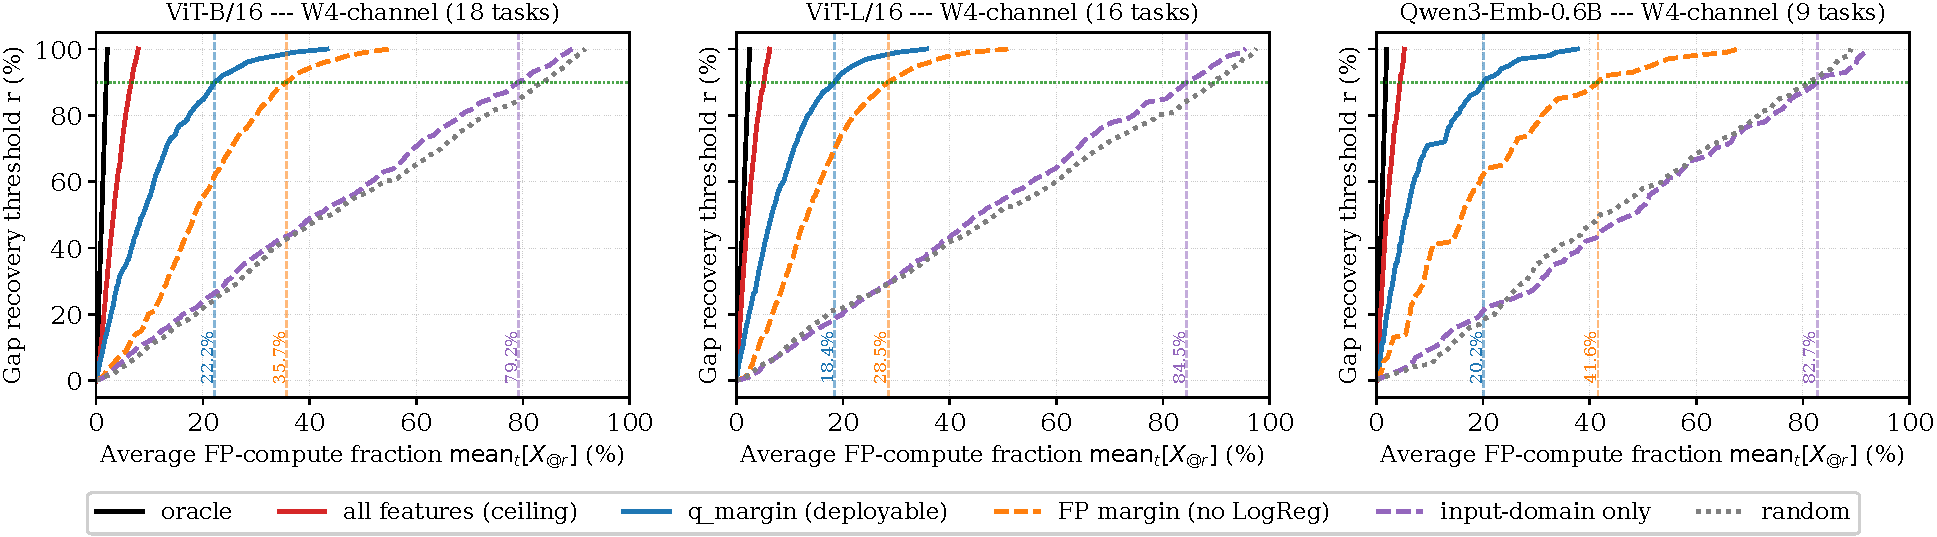
\includegraphics[width=\linewidth]{figs/fig_headline_pareto_dual_vit_base_patch16_224_orig_in21k_vs_vit_large_patch16_224_orig_in21k_bits4_channel}
\caption{\textbf{Headline Pareto at W4-channel \ptq{}.} \textbf{Left:} ViT-B/16 (18 tasks). \textbf{Center:} ViT-L/16 (16 tasks). \textbf{Right:} Qwen3-Emb-0.6B (9 NLP tasks). Each curve plots $\mathrm{mean}_t[X_{@r}(t)]$, the across-task mean of the per-task routing budget needed to recover fraction $r$ of the \fp$\to$\ptq{} gap, against $r$. The vertical dashed lines mark each method's X@90 (read at $r=0.9$); the rotated color-coded number next to each line is that X@90 value. Only the \texttt{all features (ceiling)} curve is LOO-trained (multivariate LogReg); all other curves are per-task sort-by-score.}
\label{fig:headline}
\end{figure}

\paragraph{Contributions.}
\begin{enumerate}[leftmargin=*,topsep=2pt,itemsep=2pt]
  \item \textbf{Framing input-aware PTQ routing as a tractable problem.}
        To our knowledge, no prior work routes \emph{individual inputs} between a fixed quantized model and its full-precision counterpart at deployment time without training a router: the PTQ literature targets the quantization algorithm, the selective-prediction literature targets generic model failures rather than PTQ-induced ones, and the closest precision-routing work learns a router over KV-cache chunks~\cite{tao2025moqae}. We pose the problem (predict, from cheap per-input features, which inputs PTQ will break) and provide a proof of concept that it is tractable: inputs do carry properties that predict PTQ fragility, and a single quantized-model logit margin already goes a long way.
  \item \textbf{A single PTQ margin threshold is the budget-universal optimal single-pass routing rule within the recoverable regime.} The quantized model's top-1/top-2 logit margin tracks how close an input sits to a flippable decision boundary, which the intuition in \S\ref{sec:intro} identifies as the right notion of fragility. We threshold this margin at a label-free per-task percentile; the recipe needs no training, no labels, and no fitted weights beyond calibration data. We prove that, among all scores computed from the quantized logits, the order-equivalence class of \texttt{q\_margin} (scores that preserve its strict ranking) is the only family whose level sets match the worst-case-flippable input set for \emph{every} perturbation size (Thm.~1, \S\ref{sec:theory}); a complementary hypothesis-dependent result (Prop.~2) describes when the deployable-vs-ceiling gap is structurally irreducible.
  \item \textbf{Margin matches or beats every confidence-based baseline on
        PTQ routing.} The selective-prediction / OOD-detection literature
        defaults to max-softmax-prob (MSP~\cite{hendrycks2017baseline,
        geifman2017selective}), which measures absolute confidence rather than
        boundary proximity. Our margin recipe beats MSP in all experiments at W4-channel weight-only \ptq{}, and matches the best of the multivariate confidence-based alternatives we tested. To our knowledge, neither logit margin nor MSP has been previously evaluated as a PTQ-routing signal.
   \item \textbf{Comprehensive evaluation across modalities, quantization
        granularities, and bit-widths.} Three backbones spanning two modalities
        (two ViTs and a decoder-only NLP embedding model, 53 finetuned
        classifiers in total: 21 vision tasks per ViT plus 11 NLP tasks on Qwen3), two quantization granularities (one scale per
        output channel and one scale per 128-weight group within a channel),
        and two bit-widths (4 and 3).
\end{enumerate}


% =============================================================================
\section{Related work}

\paragraph{Weight-only \ptq.}
A line of work compresses transformer weights to low bit-widths without retraining: GPTQ~\cite{frantar2023gptq}, SmoothQuant~\cite{xiao2023smoothquant}, AWQ~\cite{lin2024awq}, QuaRot~\cite{ashkboos2024quarot}, SpinQuant~\cite{liu2024spinquant}, RepQ-ViT~\cite{li2023repqvit}, PTQ4ViT~\cite{ptq4vit}, AdaLog~\cite{adalog}.
These methods target \emph{the quantization algorithm}: they change how weights are rounded so that the quantized model is closer to \fp{} on average.
Our work is orthogonal: we take a quantized model as given and target \emph{which inputs to defer}.

\paragraph{Improving the model's PTQ-robustness.}
A complementary line of work tries to make the FP model itself more amenable to subsequent \ptq{}, either by intervening on training dynamics~\cite{catalan2025training, jacob2018quantization} or by editing weights post-training without further finetuning~\cite{solombrino2026zeroshotquantizationweightspacearithmetic}. These methods change \emph{the model being quantized} so that \ptq{} damages fewer inputs. Our routing approach is orthogonal: it estimates the per-input fragility  and decides which inputs to spend \fp{} compute on.

\paragraph{Input-aware mixed precision.}
Per-layer mixed-precision quantization assigns different bit-widths to different layers~\cite{dong2019hawq}, but the decision is a one-time architectural choice, not per-input.
Cascades and early-exit networks~\cite{teerapittayanon2016branchynet,huang2018msdnet,kolawole2024revisiting} route inputs through progressively more expensive models using cheap-model confidence or ensemble agreement as the escalation signal; our work fits this template at a finer granularity (one routing decision per input, two instances of the \emph{same} model at different numerical precision) and uses cross-model disagreement features rather than confidence or agreement among differently-sized models.
MoQAE~\cite{tao2025moqae} also routes inputs across precision levels, but per \emph{chunk} via a \emph{learned} MoE router fine-tuned with a custom accuracy/memory loss, targeting KV-cache compression for long-context LLMs; our recipe is label- and training-free, and targets weight-only \ptq{} accuracy on classification.

\paragraph{Speculative decoding with quantized drafts.}
A parallel line uses the \ptq{} model as a cheap \emph{drafter} and the \fp{} model as a \emph{verifier} in speculative decoding: QSpec~\cite{zhao2025qspec} pairs complementary quantization schemes (up to 1.64$\times$ speedup), and ML-SpecQD~\cite{georganas2025mlspecqdmultilevelspeculativedecoding} uses an MXFP4 draft for a BF16 target (up to 2.72$\times$). These methods share our premise that the quantized model is right most of the time, but the \fp{} model runs on \emph{every} input as the verifier; the speedup comes from drafting and verifying multiple tokens per \fp{} pass, not from skipping \fp{}. Our routing instead avoids running \fp{} on the majority of inputs, which requires a different signal, per-input fragility, rather than per-token agreement during generation.

\paragraph{Calibration and difficulty prediction.}
A separate line of work estimates per-input difficulty from model confidence and uses it for selective classification~\cite{geifman2017selective}, abstention, or label-noise detection.
Our predictor falls in this family but is the first (to our knowledge) to explicitly aim to predict \emph{\ptq-induced} errors as distinct from generic model failures.

% =============================================================================
\section{Method}\label{sec:method}

\subsection{Setup and definitions}

Given a fixed model architecture, a finetuning task \(t\), and a \ptq scheme (e.g.\ W4-channel weight-only quantization), let \fp and \ptq be the full-precision and quantized models respectively.
For each test input \(x\) with gold label \(y\), define:
\begin{align}
  \text{good}(x) &:= \mathbf{1}\!\left[\fp(x)\!=\!y \wedge \ptq(x)\!=\!y\right]\\
  \text{bad}(x)  &:= \mathbf{1}\!\left[\fp(x)\!=\!y \wedge \ptq(x)\!\neq\!y\right]\\
  \text{lucky-Q}(x) &:= \mathbf{1}\!\left[\fp(x)\!\neq\!y \wedge \ptq(x)\!=\!y\right]
\end{align}

Routing an input \(x\) to \fp{} changes its correctness by \(+1\) if \(\text{bad}(x)\), \(-1\) if \(\text{lucky-Q}(x)\), and 0 otherwise.
The \emph{oracle score} is therefore exactly \(\text{bad}(x)-\text{lucky-Q}(x)\).
A practical predictor must approximate this score from features available before the label is known.

\subsection{Routing recipe}\label{sec:routing_recipe}

\paragraph{The score.}
Our routing score is the quantized model's top-1/top-2 logit margin,
\[
  \mathrm{q\_margin}(x) \;:=\; \ptq_{(1)}(x) - \ptq_{(2)}(x),
\]
where $\ptq_{(k)}$ is the $k$-th largest logit. This is a single scalar from a single \ptq{} forward pass, no extra compute beyond what \ptq{} inference already performs. Low margin = boundary-close = PTQ-fragile. No labels are used at deployment.

\paragraph{Batch routing.} sorts the test set by ascending $\mathrm{q\_margin}$ and routes the bottom $X\%$ of inputs (i.e., the lowest-margin inputs) to \fp{}. Output: the routed accuracy at every $X$. The smallest $X$ such that the routed accuracy recovers fraction $R$ of the \fp$\to$\ptq{} gap is denoted \xat{R} (we write \xat{90} or just ``X@90'' for $R\!=\!0.9$ throughout; the headline metric is the per-task \xat{90} averaged across eligible tasks). Batch routing requires the test set to be sorted before routing.

\paragraph{Online routing.} commits to a fixed threshold $\tau$: each new input $x$ is routed to FP iff $\mathrm{q\_margin}(x) < \tau$. The threshold is set on the target task's \emph{validation split}, a small slice of the data held out from finetuning and disjoint from the test set used for evaluation, so the test inputs are never seen at calibration time. Our headline recipe is the \emph{label-free} \texttt{val\_pct}; when the deployer happens to have labels on the calibration slice, we additionally offer a stronger label-aware variant \texttt{val\_x90}.
\begin{itemize}[leftmargin=*,topsep=2pt,itemsep=0pt]
  \item \texttt{val\_pct} (label-free, main): set $\tau$ at the 25th percentile of $\mathrm{q\_margin}$ on the target's \emph{unlabeled} validation set. The 25\% is a single global hyperparameter, defensible \emph{a priori} (a typical PTQ-broken fraction is a few percent, with imperfect ranking the routing budget should be a small multiple of that) rather than tuned per task.
  \item \texttt{val\_x90} (label-aware variant, optional): when calibration labels are available, find the smallest per-task $\tau$ such that routing the resulting fraction on the labeled val set recovers $\geq$\,90\% of the val \fp$\to$\ptq{} gap; apply that $\tau$ to test. No global hyperparameter is needed. Applicable as an alternative for deployers with labeled calibration data.
\end{itemize}
Both recipes are deployable: $\tau$ is fixed before any test input arrives, and each test input is decided individually without seeing other test inputs. The label-free claim rests on \texttt{val\_pct} alone; \texttt{val\_x90} is included for completeness because labeled validation data is often available in practice (deployment already requires finetuning, which requires labels), but it is not required to deploy the recipe.

\paragraph{Baselines.}
The \emph{max-softmax probability} (MSP) baseline uses the same recipe with the score replaced by $-\max(\mathrm{softmax}(\ptq(x)))$. We additionally evaluate single-feature variants ($-\mathrm{entropy}$), pairwise combinations, and a per-task-z-scored logistic regression over the full feature universe, Q-side (margin, MSP, entropy), \fp{}-side scalars from one \fp{} forward pass, four image-pixel input-domain statistics on ViTs (brightness = mean, contrast = std, edge density = Sobel-magnitude mean, FFT high-frequency ratio = fraction outside the 0.25-Nyquist disk) or four tokenizer-side text statistics on Qwen3 (\texttt{txt\_n\_tokens}, \texttt{txt\_n\_unique\_tokens}, \texttt{txt\_type\_token\_ratio}, \texttt{txt\_punct\_ratio}), and cross-model features (logit/softmax at the other model's predicted class, symmetric KL between softmax distributions, the $\fp\!\neq\!\ptq$ disagreement flag; require both forward passes per input). These are reported as ablations in \S\ref{sec:ablation}.

\paragraph{All baselines reduce to a per-input continuous score.}
Every baseline produces one scalar per input, then plugs into the same batch- and online-routing procedures defined above for \texttt{q\_margin}: batch sorts by the score and routes the bottom $X\%$; online thresholds the score at a pre-set $\tau$. No baseline produces a hard classification. Concretely, the score is the feature value itself for singleton baselines (e.g., \texttt{q\_margin\_only}, \texttt{msp\_only}), $P(\bad)$ from a LogReg fit on the named feature set for multivariate baselines (e.g., \texttt{q\_only}, \texttt{all\_features}), $\text{bad}(x) - \text{lucky-Q}(x)$ for the \emph{oracle}, and an i.i.d.\ uniform draw for \emph{random}. App.~\ref{app:baselines_indepth} unpacks each named baseline subset, including which features go into it, what its score means, and why we include it.

\paragraph{LOO protocol for multivariate ablations.}
Our single-feature recipe needs no training. However, the multivariate logistic-regression baseline requires training, and we use leave-one-out (LOO) cross-task transfer: for each held-out target task $t^\ast$, train on the pooled validation \fp{}-correct rows of every other task with per-task z-scoring, and score the held-out target's validation and test. This isolates the question of whether one fitted predictor can deploy across tasks without per-task retraining.

\subsection{Theoretical optimality of \texttt{q\_margin}}\label{sec:theory}

We now show that the empirical superiority of \texttt{q\_margin} reflects a precise minimax-optimality property, paired with a matching information-theoretic limit that explains the gap between the deployable recipe and the diagnostic ceiling. Full proofs are deferred to App.~\ref{app:proofs}.

\paragraph{Notation.}
Throughout this subsection, $\ptq(x) \in \mathbb R^C$ denotes the $C$-dimensional logit vector of the quantized model at input $x$, and $\arg\max\ptq(x)$ its predicted class (the predicate use of $\ptq(x)$ in \S\ref{sec:method}, e.g.\ ``$\ptq(x)\!=\!y$'', refers to the latter). Fix a perturbation budget $\epsilon > 0$: by this we mean an $L_\infty$ bound on the additive \emph{logit} perturbation $\widetilde{\ptq}(x) - \ptq(x)$ of an arbitrary perturbed classifier $\widetilde{\ptq}$, with $\|v\|_\infty := \max_k |v_k|$. Intuitively, $\widetilde{\ptq}$ stands in for the end-to-end effect of any weight-only \ptq{} rounding whose logit-space deviation is bounded by $\epsilon$. All probabilities $\Pr_x[\cdot]$ are taken under the task's test-input distribution. Let $D := \{x : \arg\max\fp(x) \neq \arg\max\ptq(x)\}$ denote the \fp{}/\ptq{} \emph{disagreement set}.

\paragraph{Proposition 1 (Margin perturbation bound).}
\emph{Let $\widetilde{\ptq}$ be any classifier with $\|\widetilde{\ptq}(x) - \ptq(x)\|_\infty \leq \epsilon$. If $\mathrm{q\_margin}(x) > 2\epsilon$, then $\arg\max\widetilde{\ptq}(x) = \arg\max\ptq(x)$.}

Define the \emph{flippable set} $\mathcal F_\epsilon := \{x : \mathrm{q\_margin}(x) < 2\epsilon\}$: by Proposition~1 and a matching converse (App.~\ref{app:proofs}), this is exactly the set of inputs whose \ptq{} prediction can be flipped by \emph{some} $L_\infty$-bounded perturbation of size $\leq\epsilon$.

\paragraph{Theorem 1 (Budget-universal optimality of \texttt{q\_margin}).}
\emph{Let $\mathcal S$ be the class of measurable scoring functions of the form $s(x) = g(\ptq(x))$ for some $g : \mathbb R^C \to \mathbb R$, and assume $\mathrm{q\_margin}$ has an atom-free distribution under $\Pr_x$. Under the routing convention of \S\ref{sec:routing_recipe} (lower $s(x)$ means higher routing priority), the following are equivalent for $s \in \mathcal S$:}

\emph{(i) For every $\epsilon > 0$ there exists a threshold $\theta_\epsilon \in \mathbb R$ such that the routed set $\{x : s(x) \leq \theta_\epsilon\}$ equals the flippable set $\mathcal F_\epsilon$ up to a $\Pr_x$-null set.}

\emph{(ii) $s$ preserves the strict order of $\mathrm{q\_margin}$: for $\Pr_x \otimes \Pr_x$-almost every pair $(x, x')$,
\[
\mathrm{q\_margin}(x) < \mathrm{q\_margin}(x') \;\implies\; s(x) < s(x').
\]
}

\emph{In particular, $s = \mathrm{q\_margin}$ satisfies (ii) (and hence (i) via $\theta_\epsilon = 2\epsilon$), and any score whose ranking disagrees with $\mathrm{q\_margin}$ on a set of pairs of positive measure fails (i) at some perturbation budget.}

In words: among all routing scores computed from the quantized logits, only those that share \texttt{q\_margin}'s strict ranking on almost every pair of inputs match the worst-case-flippable sets \emph{across all perturbation budgets simultaneously}. A deployer who does not know the perturbation size $\epsilon$ in advance therefore has a unique best-effort single-pass ranking: order inputs by \texttt{q\_margin}. Any other \ptq-logit-derived score that re-ranks a positive-measure set of pairs against \texttt{q\_margin} fails the optimum at some $\epsilon$. The recipe's empirical superiority over MSP, entropy, and FP-side multivariate baselines (\S\ref{sec:ablation}) is consistent with this: none of those scores is order-equivalent to \texttt{q\_margin}, so they cannot match its level sets across budgets. Theorem~1 is a worst-case (adversarial-perturbation) statement, but its quantifier ``for every $\epsilon$'' is what gives \texttt{q\_margin} its uniqueness: the deployer commits to a single ranking before knowing the rounding magnitude. \emph{Scope.} Theorem~1 covers scores computed from the \ptq{} logit vector; input-domain features (image-pixel statistics, tokenizer-side statistics) are formally outside its scope, but the empirical ablation finds them near chance (Table~\ref{tab:univariate}), providing independent evidence that they do not add routing signal.

\paragraph{Proposition 2 (Single-pass information limit).}
\emph{Suppose the data distribution satisfies a symmetry on $D$: the conditional distribution of $\ptq(x)$ given $\bad(x)\!=\!1$ matches that given $\luckyq(x)\!=\!1$ ($\bad$ and $\luckyq$ are disjoint sub-events of $D$). Then for any measurable $s: \mathbb R^C \to \mathbb R$, the AUROC of $s(\ptq(x))$ as a discriminator between $\bad$ and $\luckyq$ (on $\bad \cup \luckyq$) equals $\tfrac12$.}

The symmetry hypothesis is stronger than ``both populations sit near \ptq's decision boundary'': it asks the full conditional distribution of $\ptq(x)$ to coincide on $\bad$ and $\luckyq$ inputs. We cannot verify this on real data, so Proposition~2 should be read as a conditional impossibility result: it identifies a regime in which the deployable-vs-ceiling gap would be structurally irreducible without cross-model features. The empirical gap ($\approx$\,22\% vs $\approx$\,7.5\% on ViT-B/16) is \emph{consistent with} this hypothesis being approximately satisfied; whether the gap can be partly closed by some cleverer \ptq-logit-derived score that exploits a violation of the symmetry remains open.

\paragraph{Combined characterization.}
Theorem~1 says the order-equivalence class of \texttt{q\_margin} is the unique family of budget-universal scores for \emph{catching} the inputs that bounded \ptq{} rounding could flip; Proposition~2 says that under a symmetry hypothesis on the \bad{}/\luckyq{} populations, no \ptq-logit-derived score can \emph{resolve} which catches are worth routing. Together they bracket the recipe's empirical Pareto: \texttt{q\_margin}'s \xat{90} is as low as any \ptq-logit-derived score can go uniformly across perturbation budgets (Thm.~1), and the gap to the diagnostic ceiling is consistent with --- though not proved by --- a structural single-pass-information limit (Prop.~2).

% =============================================================================
\section{Experimental setup}\label{sec:setup}

\paragraph{Backbones and tasks.}
We evaluate three backbones: two ViTs, \texttt{ViT-B/16} and \texttt{ViT-L/16}~\cite{dosovitskiy2021image} loaded from the timm library~\cite{rw2019timm}, each finetuned on the same 21 vision classification tasks (natural images, satellite imagery, digits, fine-grained categories, faces, rendered text; see Appendix~\ref{app:tasks}); and \texttt{Qwen3-Embedding-0.6B}~\cite{zhang2025qwen3}, a decoder-only embedding model wrapped via HuggingFace's \texttt{AutoModelForSequenceClassification}, finetuned on 11 standard NLP classification tasks drawn from the MTEB benchmark~\cite{muennighoff2023mteb}: Banking77~\cite{casanueva-etal-2020-efficient}, Emotion~\cite{saravia-etal-2018-carer}, IMDB~\cite{maas-etal-2011-learning}, MTOPDomain/Intent~\cite{li-etal-2021-mtop}, MassiveIntent/Scenario~\cite{fitzgerald2022massive}, AmazonCounterfactual~\cite{oneill-etal-2021-wish}, AmazonReviewsClassification~\cite{keung2020multilingual}, ToxicConversations~\cite{jigsaw-unintended-bias-in-toxicity-classification}, TweetSentimentExtraction~\cite{tweet-sentiment-extraction}. On the vision side, the input-domain features are four image-pixel statistics (\S\ref{sec:ablation}, Table~\ref{tab:univariate}); on Qwen3 they are replaced by four tokenizer-side text statistics (\texttt{txt\_n\_tokens}, \texttt{txt\_n\_unique\_tokens}, \texttt{txt\_type\_token\_ratio}, \texttt{txt\_punct\_ratio}). All other features (Q-side, FP-side, cross-model) are identical across backbones.
All finetunes share hyperparameters except batch size, which is 128 for ViT-B and 64 for ViT-L (full list in App.~\ref{app:hp}). Validation/test splits are deterministic with \(\textsc{SPLIT\_SEED}\!=\!0\), \(\text{VAL\_FRACTION}\!=\!0.1\) capped at 5000 samples.

\paragraph{\ptq{} regimes.}
The primary regime is weight-only W4-channel \ptq{} by naive round-to-nearest (RTN), applied to every linear layer except the head (\texttt{skip\_modules=[head]} on ViT, \texttt{skip\_modules=[score]} on Qwen3); we also evaluate at W3-channel as a stress test. RTN is the weakest weight-only \ptq{}; we use it deliberately as a controlled setting (\S\ref{sec:discussion}).
The same regime is applied identically across all three backbones.

\paragraph{Eligibility filter.}
A task is included in the W4-channel analysis only if \ptq{} produces at least 10 \bad{} samples on both validation and test; otherwise the per-task \xat{90} estimate is too noisy to be meaningful.
\textbf{For ViT-B/16}, 3 tasks fail this filter (Flowers102, OxfordIIITPet, STL10): all three are tasks where W4-channel \ptq{} barely degrades the ViT-B/16 finetune.
\textbf{For ViT-L/16}, 5 tasks fail (those three plus EuroSAT and GTSRB): ViT-L/16's extra capacity preserves \emph{more} inputs under PTQ, so the recoverable regime is narrower at scale.
\textbf{For Qwen3}, 2 of 11 tasks fail (AmazonCounterfactual and MTOPDomain, both at $\approx$ 95\% FP accuracy where PTQ barely degrades).
The W4-channel analysis therefore runs on 18 tasks for ViT-B/16, 16 for ViT-L/16, and 9 for Qwen3.
At W3-channel all tasks are eligible on all three backbones, because PTQ produces large numbers of \bad{} samples on every task there.

% =============================================================================
\section{Results}\label{sec:results}

\subsection{The margin recipe}\label{sec:headline}

\paragraph{Univariate feature AUC.}
Before evaluating multivariate routing scores, we ask which individual features can discriminate \bad{} inputs from \good{} ones. For each feature we report its ROC-AUC against the \bad{}-vs-\good{} label on FP-correct validation rows, the population where routing actually matters, folded as $\max(\mathrm{AUC},\,1-\mathrm{AUC})$ so the score is sign-agnostic. Two groups emerge cleanly: model-derived margin/softmax/entropy features on either the \fp{} or \ptq{} side are strongly discriminative (mean AUC 0.83--0.94 on ViT-B/16), while the four image-pixel statistics (brightness, contrast, edge density, FFT high-frequency ratio) hover at chance ($\approx 0.54$). This previews the multivariate result below: surface image and text features cannot rescue routing on their own, and the model-derived features are individually strong enough that combining them adds little. Full per-feature breakdown in Appendix~\ref{app:univariate}.

% Auto-generated by code/visualizations/.../004_input_fragility/generate_paper_tables.py
% Dual-backbone ablation: vit_base_patch16_224_orig_in21k & vit_large_patch16_224_orig_in21k, W4 and W3 (channel).
\begin{table}[t]
\centering
\caption{\xat{90} per feature subset on ViT-B/16 and ViT-L/16 at W4-channel and W3-channel. Lower is better. Singleton and pairwise rows are per-task sort-by-score (no fitted classifier); the multivariate rows (\texttt{q\_only}, \texttt{fp\_only}, \texttt{fp\_plus\_q\_no\_cross}, \texttt{all\_features}) use a leave-one-out (LOO) cross-task LogReg. Eligible-task counts in the last row.}
\label{tab:ablation}
\small
\setlength{\tabcolsep}{4pt}
\begin{tabular}{llcccc}
\toprule
& & \multicolumn{2}{c}{W4-channel} & \multicolumn{2}{c}{W3-channel} \\
\cmidrule(lr){3-4} \cmidrule(lr){5-6}
Subset & Deployment & ViT-B/16 & ViT-L/16 & ViT-B/16 & ViT-L/16 \\
\midrule
\texttt{image\_only} & no model & 79.2 $\pm$ 17.4 & 84.5 $\pm$ 8.3 & 86.4 $\pm$ 9.5 & 88.3 $\pm$ 4.3 \\
\texttt{msp\_only} & MSP baseline & 30.4 $\pm$ 24.3 & 22.0 $\pm$ 16.5 & 81.0 $\pm$ 10.3 & 83.3 $\pm$ 14.6 \\
\texttt{q\_margin\_only} & margin (proposed) & 22.2 $\pm$ 17.2 & 18.4 $\pm$ 12.0 & 81.7 $\pm$ 10.6 & 83.8 $\pm$ 14.7 \\
\texttt{q\_entropy\_only} & entropy alone & 41.5 $\pm$ 32.5 & 27.7 $\pm$ 21.1 & 81.9 $\pm$ 10.5 & 83.4 $\pm$ 14.6 \\
\texttt{q\_margin\_msp} & margin + MSP & 22.5 $\pm$ 18.3 & 18.3 $\pm$ 11.5 & 81.1 $\pm$ 10.3 & 83.4 $\pm$ 14.6 \\
\texttt{q\_margin\_entropy} & margin + entropy & 24.0 $\pm$ 18.5 & 18.6 $\pm$ 12.1 & 81.4 $\pm$ 10.4 & 83.4 $\pm$ 14.6 \\
\texttt{q\_msp\_entropy} & MSP + entropy & 26.5 $\pm$ 22.3 & 19.0 $\pm$ 13.1 & 81.1 $\pm$ 10.3 & 83.3 $\pm$ 14.6 \\
\texttt{q\_only} & all 3 Q-side (LogReg) & 24.4 $\pm$ 20.8 & 18.2 $\pm$ 11.9 & 81.2 $\pm$ 10.3 & 83.4 $\pm$ 14.6 \\
\texttt{fp\_only} & FP-side only & 34.9 $\pm$ 23.1 & 26.9 $\pm$ 16.6 & 90.5 $\pm$ 3.4 & 88.7 $\pm$ 5.5 \\
\texttt{fp\_plus\_q\_no\_cross} & both models & 25.8 $\pm$ 20.9 & 18.9 $\pm$ 13.4 & 82.7 $\pm$ 7.3 & 83.8 $\pm$ 13.5 \\
\texttt{all\_features} & ceiling (both+cross) & 7.5 $\pm$ 8.8 & 6.0 $\pm$ 5.1 & 65.7 $\pm$ 16.9 & 70.9 $\pm$ 19.6 \\
\midrule
oracle & oracle (upper bound) & 1.9 $\pm$ 1.4 & 2.3 $\pm$ 2.2 & 53.8 $\pm$ 16.7 & 66.5 $\pm$ 20.1 \\
random & random (lower bound) & 83.8 $\pm$ 21.5 & 89.8 $\pm$ 2.8 & 90.3 $\pm$ 1.2 & 89.4 $\pm$ 2.5 \\
\midrule
\multicolumn{2}{r}{$n_{\text{eligible tasks}}$} & 18 & 16 & 21 & 21 \\
\bottomrule
\end{tabular}
\end{table}


\begin{table}[t]
\centering
\caption{\textbf{Qwen3 ablation, companion to Table~\ref{tab:ablation}.} \xat{90} per feature subset on Qwen3-Emb-0.6B. Lower is better. Same row taxonomy as Table~\ref{tab:ablation}: singleton/pairwise rows are per-task sort-by-score; multivariate rows (\texttt{q\_only}, \texttt{fp\_only}, \texttt{fp\_plus\_q\_no\_cross}, \texttt{all\_features}) use LOO cross-task LogReg. Eligible task counts in the last row.}
\label{tab:qwen3}
\small
\setlength{\tabcolsep}{5pt}
\begin{tabular}{llcc}
\toprule
Subset & Deployment & W4-channel & W3-channel \\
\midrule
\texttt{text\_only}             & no model               & 82.7 $\pm$ 18.1 & 89.6 $\pm$ 1.9 \\
\texttt{msp\_only}              & MSP baseline           & 21.0 $\pm$ 16.5 & 83.3 $\pm$ 12.3 \\
\texttt{q\_margin\_only}        & margin (proposed)      & 20.2 $\pm$ 16.5 & 83.4 $\pm$ 12.3 \\
\texttt{q\_entropy\_only}       & entropy alone          & 21.2 $\pm$ 16.1 & 83.3 $\pm$ 12.3 \\
\texttt{q\_margin\_msp}         & margin + MSP           & 20.3 $\pm$ 16.5 & 83.3 $\pm$ 12.3 \\
\texttt{q\_margin\_entropy}     & margin + entropy       & 20.5 $\pm$ 16.4 & 83.3 $\pm$ 12.3 \\
\texttt{q\_msp\_entropy}        & MSP + entropy          & 24.0 $\pm$ 15.0 & 83.3 $\pm$ 12.3 \\
\texttt{q\_only}                & all 3 Q-side (LogReg)  & 20.8 $\pm$ 16.2 & 83.3 $\pm$ 12.3 \\
\texttt{fp\_only}               & FP-side only           & 41.6 $\pm$ 21.2 & 90.0 $\pm$ 1.0 \\
\texttt{fp\_plus\_q\_no\_cross} & both models            & 25.1 $\pm$ 18.6 & 82.3 $\pm$ 14.3 \\
\texttt{all\_features}          & ceiling (both+cross)   & 6.0 $\pm$ 3.6   & 57.3 $\pm$ 24.4 \\
\midrule
oracle                          & oracle (upper bound)   & 1.8 $\pm$ 1.1   & 50.0 $\pm$ 26.0 \\
random                          & random (lower bound)   & 80.9 $\pm$ 21.1 & 90.0 $\pm$ 0.6 \\
\midrule
\multicolumn{2}{r}{$n_{\text{eligible tasks}}$} & 9 & 11 \\
\bottomrule
\end{tabular}
\end{table}

\paragraph{Pareto routing curves.}
Figure~\ref{fig:headline} plots $\mathrm{mean}_t[X_{@r}(t)]$ vs.\ gap-recovery threshold $r$ for the headline scores on all three backbones; Table~\ref{tab:ablation} reads off \xat{90} (the smallest \fp{}-compute fraction at which routing recovers 90\% of the \fp$\to$\ptq{} gap) for each feature subset on both vision backbones and at both \ptq{} regimes.

The \texttt{q\_margin} score has an offline X@90 of 18--22\%. Specifically, under W4-channel PTQ, sorting by \texttt{q\_margin} gives an offline X@90 of \textbf{22.2\% on ViT-B/16}, \textbf{18.4\% on ViT-L/16}, and \textbf{20.2\% on Qwen3}: these are the smallest per-task FP-compute fractions at which an offline sort by \texttt{q\_margin} recovers 90\% of the \fp$\to$\ptq{} gap, averaged across eligible tasks. They are several times better than the random baseline ($\sim$84\%/$\sim$90\%/$\sim$81\%). The score costs nothing beyond the single \ptq{} forward pass that the deployment is already doing. \S\ref{sec:online} shows how a label-free online recipe approximates the offline X@90 budget at deployment  time. The next subsection asks whether anything else can match or beat the offline X@90 of \texttt{q\_margin}: alternative confidence signals, multivariate combinations, FP-side clues, or input-domain features.

\subsection{Baselines comparisons: nothing outperforms \texttt{q\_margin}}\label{sec:ablation}

\paragraph{Baseline 1: MSP, the canonical confidence signal.}
The selective-prediction / OOD-detection literature defaults to thresholding the quantized model's top-1 softmax probability (MSP~\cite{hendrycks2017baseline,geifman2017selective}). MSP recovers 90\% of the gap at 30.4\%/22.0\%/21.0\% routing on the three backbones (\texttt{msp\_only}, Table~\ref{tab:ablation}), worse than \texttt{q\_margin}by 8.2/3.6/0.8 pp. The mechanism predicts this gap: MSP measures absolute top-1 confidence, while the decision-boundary failure depends on top-1 vs.\ top-2 separation.

\paragraph{Baseline 2: other Q-side features and pairwise combinations.}
Entropy alone (\texttt{q\_entropy\_only}: 41.5\%/27.7\%/21.2\%) is the weakest Q-side singleton; entropy carries little signal in isolation. Pairing \texttt{q\_margin}with MSP (\texttt{q\_margin\_msp}), with entropy (\texttt{q\_margin\_entropy}), or with both (\texttt{q\_only}, the 3-feature Q-side logistic regression) leaves \xat{90} statistically indistinguishable from \texttt{q\_margin} alone on every backbone, and on ViT-B/16 the 3-feature LogReg, which includes \texttt{q\_margin}, actually even hurts slightly. Combinations that drop \texttt{q\_margin} (\texttt{q\_msp\_entropy}: 26.5\%/19.0\%/24.0\%) are uniformly worse, confirming \texttt{q\_margin} as the load-bearing feature. The Q-side ceiling is reached by a single feature; no fitted model is needed.

\paragraph{Baseline 3: FP-side, input-domain, and cross-model features.}
The \texttt{fp\_only} baseline (\fp{}-side scalars only) reaches \xat{90} $=$ 34.9\% on ViT-B/16 and 26.9\% on ViT-L/16, worse than \texttt{q\_margin\_only} by $\sim$1.5$\times$ on both backbones (mechanism discussed in \S\ref{sec:discussion}). Adding image-pixel or tokenizer-side text statistics to either Q-only or FP-only changes nothing; these descriptors carry no measurable signal (per-feature AUC $\approx$ 0.54 on ViT-B/16, Appendix~\ref{app:univariate}; \texttt{text\_only} subset reaches AUROC 0.494 on Qwen3, Table~\ref{tab:qwen3}). The only configuration that closes the gap to oracle is the full \texttt{all\_features} set (7.5\% / 6.0\% / 6.0\% on the three backbones, close to oracle's 1.9\% / 2.3\% / 1.8\%), but at the cost of running both the \fp{} and \ptq{} models on every input, which loses the point since it already runs the FP model. We report it as a \emph{diagnostic ceiling}, not a deployable recipe. The \texttt{all\_features} AUROC is suppressed in Table~\ref{tab:auroc} due to a definitional label leak via the disagreement feature; this leak does not affect the \xat{90} number because that metric is computed over the full test set (App.~\ref{app:auroc_leak}). Figure~\ref{fig:ablation} shows the full Pareto curves per feature subset.

\begin{figure}[t]
\centering
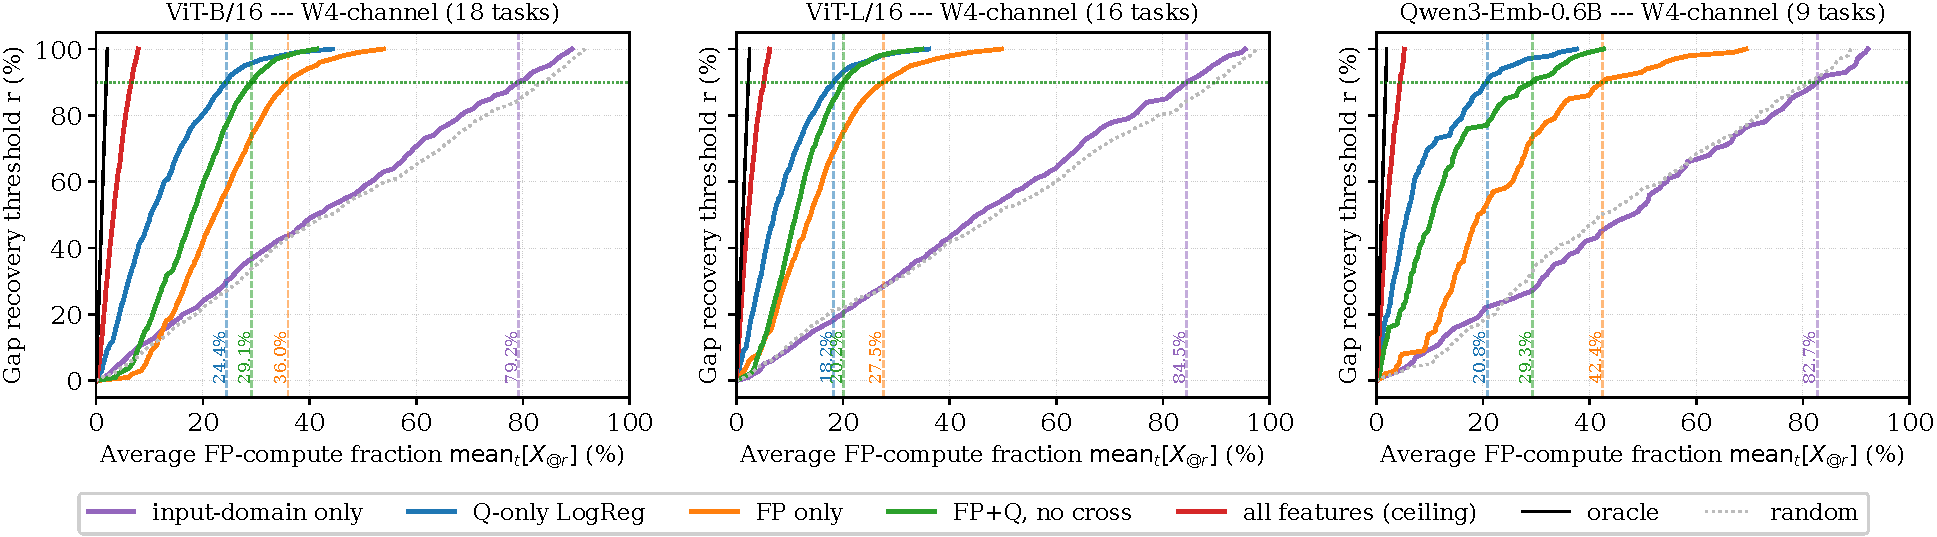
\includegraphics[width=\linewidth]{figs/fig_feature_ablation_dual_vit_base_patch16_224_orig_in21k_vs_vit_large_patch16_224_orig_in21k_bits4_channel}
\caption{\textbf{Multivariate feature ablation at W4-channel.} Same axes and aggregation as Figure~\ref{fig:headline}, one curve per feature subset. \textbf{Left:} ViT-B/16. \textbf{Center:} ViT-L/16. \textbf{Right:} Qwen3-Emb-0.6B. Multivariate LogReg subsets (\texttt{Q-only LogReg}, \texttt{FP only}, \texttt{FP+Q no cross}, \texttt{all features}) are LOO-trained; \texttt{oracle}, \texttt{random}, and \texttt{input-domain only} are per-task sort-by-score (shared with Figure~\ref{fig:headline}).}
\label{fig:ablation}
\end{figure}

The gap between the deployable \texttt{q\_margin} recipe and the diagnostic ceiling is mechanism-grounded in the \emph{\luckyq{} ambiguity} (\S\ref{sec:discussion}).

\paragraph{Multivariate LogReg ablation: cross-task generalization.}
The single-feature \texttt{q\_margin} recipe needs no training, so cross-task generalization is only a concern for the multivariate LogReg ablations above, which in any case do not significantly improve on \texttt{q\_margin} alone. For completeness: when we do fit a LogReg (e.g., on the 3 Q-side features), training on the pooled validation\fp{}-correct rows of all \emph{other} tasks (LOO) lands within $\sim$2.5 pp of a same-task fit on the aggregate and within $\sim$10 pp on every individual task on ViT-B/16, with tighter dispersion on ViT-L/16 (Figure~\ref{fig:loo_vs_same}, per-task table in Appendix~\ref{app:loo_per_task}). The all-features cross-model ceiling under LOO reaches \xat{90} $=$ 7.5\% / 6.0\%, an analysis tool only since it requires running both models per input.

\paragraph{Secondary metric: AUROC of the routing score on FP-correct test rows.}
The \xat{90} metric routes the entire test set and reports the resulting accuracy, which is the deployment-faithful number. As a complementary check we report AUROC, computed only on FP-correct test rows. The restriction is definitional: \bad{} and \good{} are both labels on FP-correct inputs (\S\ref{sec:method}), so AUROC of $P(\bad)$ against the \bad{}/\good{} label is only well-defined there; on FP-wrong rows the label does not exist. A threshold-free, gap-magnitude-independent metric (Table~\ref{tab:auroc}) corroborates the \xat{90} ordering: \texttt{q\_margin} reaches AUROC $\approx$ 0.94 / 0.95 / 0.92 on ViT-B/16, ViT-L/16, and Qwen3 respectively, edging MSP's 0.90 / 0.93 / 0.92 by the gap the boundary mechanism predicts. \texttt{image\_only} hovers at $\approx$ 0.51 (chance). \texttt{all\_features}'s AUROC is suppressed because the \texttt{fp\_q\_disagree} feature definitionally equals \bad{} on FP-correct rows (see Appendix~\ref{app:auroc_leak} for the leak mechanism and why the \xat{90} number remains valid). Note one consequence of the asymmetry: AUROC does not see the \luckyq{} population at all, so it cannot speak to whether the score also avoids sending \luckyq{} inputs to \fp{}; that cost is what the \xat{90}-vs-ceiling gap (\S\ref{sec:discussion}) measures.

% Auto-generated by code/visualizations/.../004_input_fragility/generate_paper_tables.py
% 3-backbone AUROC at W4-channel.
\begin{table}[t]
\centering
\caption{\textbf{AUROC of $P(\bad)$ vs \bad{} labels on FP-correct test rows} at W4-channel, per feature subset, on ViT-B/16, ViT-L/16, and Qwen3-Emb-0.6B. Higher is better. Mean $\pm$ std across eligible tasks per backbone. Singleton/pairwise rows are per-task sort-by-score; multivariate rows (\texttt{q\_only}, \texttt{fp\_only}, \texttt{fp\_plus\_q\_no\_cross}, \texttt{all\_features}) use LOO cross-task LogReg. \texttt{all\_features}'s AUROC is suppressed (---); see App.~\ref{app:auroc_leak}.}
\label{tab:auroc}
\small
\setlength{\tabcolsep}{5pt}
\begin{tabular}{llccc}
\toprule
Subset & Deployment & ViT-B/16 & ViT-L/16 & Qwen3-Emb-0.6B \\
\midrule
\texttt{image\_only / text\_only} & no model & 0.515 $\pm$ 0.042 & 0.521 $\pm$ 0.056 & 0.494 $\pm$ 0.054 \\
\texttt{msp\_only} & MSP baseline & 0.898 $\pm$ 0.082 & 0.933 $\pm$ 0.053 & 0.921 $\pm$ 0.066 \\
\texttt{q\_margin\_only} & margin (proposed) & 0.937 $\pm$ 0.043 & 0.952 $\pm$ 0.031 & 0.922 $\pm$ 0.064 \\
\texttt{q\_entropy\_only} & entropy alone & 0.807 $\pm$ 0.186 & 0.901 $\pm$ 0.082 & 0.919 $\pm$ 0.063 \\
\texttt{q\_margin\_msp} & margin + MSP & 0.937 $\pm$ 0.042 & 0.952 $\pm$ 0.031 & 0.922 $\pm$ 0.065 \\
\texttt{q\_margin\_entropy} & margin + entropy & 0.927 $\pm$ 0.050 & 0.951 $\pm$ 0.031 & 0.922 $\pm$ 0.064 \\
\texttt{q\_msp\_entropy} & MSP + entropy & 0.918 $\pm$ 0.074 & 0.947 $\pm$ 0.033 & 0.908 $\pm$ 0.058 \\
\texttt{q\_only} & all 3 Q-side (LogReg) & 0.925 $\pm$ 0.062 & 0.951 $\pm$ 0.033 & 0.921 $\pm$ 0.064 \\
\texttt{fp\_only} & FP-side only & 0.914 $\pm$ 0.064 & 0.937 $\pm$ 0.042 & 0.904 $\pm$ 0.063 \\
\texttt{fp\_plus\_q\_no\_cross} & both models & 0.930 $\pm$ 0.064 & 0.957 $\pm$ 0.032 & 0.942 $\pm$ 0.047 \\
\texttt{all\_features} & ceiling (both+cross) & --- & --- & --- \\
\midrule
\multicolumn{2}{r}{$n_{\text{eligible tasks}}$} & 18 & 16 & 9 \\
\bottomrule
\end{tabular}
\end{table}


\begin{figure}[t]
\centering
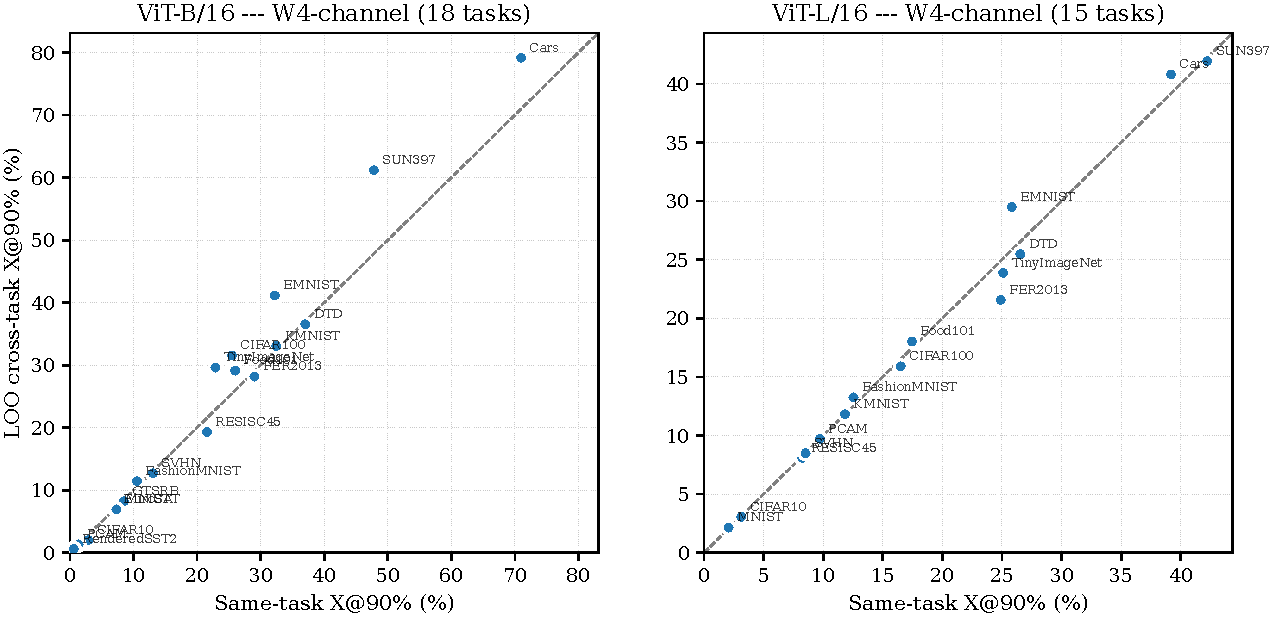
\includegraphics[width=\linewidth]{figs/fig_loo_vs_same_task_dual_vit_base_patch16_224_orig_in21k_vs_vit_large_patch16_224_orig_in21k_bits4_channel}
\caption{\textbf{LOO vs same-task \xat{90} for the 3-feature Q-only LogReg at W4-channel.} \textbf{Left:} ViT-B/16. \textbf{Right:} ViT-L/16. Each point is one task; x-axis is \xat{90} for a LogReg fit on the target's own val (same-task), y-axis is \xat{90} for a LogReg fit on every other task pooled (LOO). Points on the diagonal mean LOO equals same-task.}
\label{fig:loo_vs_same}
\end{figure}

\subsection{Robustness across scale and recipe}
\label{sec:regime}

We stress-test the recipe along three axes: backbone scale (ViT-B vs.\ ViT-L), bit-width (W4 vs.\ W3), and PTQ granularity (per-channel vs.\ per-group\_128). We summarize the headline findings here; the full per-axis analysis, the regime-polarization figure, and the per-channel vs.\ per-group\_128 comparison table are in App.~\ref{app:regime}.
First, \texttt{q\_margin} is scale-robust: its offline X@90 stays in 18--22\% across all three backbones at W4-channel.
Second, at W3 under per-channel round-to-nearest (RTN), PTQ damages the strict majority of inputs ($\sim$62\% on ViT-B/16, $\sim$75\% on ViT-L/16), the oracle's X@90 climbs to 54--67\%, and the cheap-default-with-fallback deployment shape stops applying. This is a property of the regime, not the predictor.
Third, switching to a per-group\_128 RTN refinement (one scale per 128-weight block, same naive rounding, no calibration or runtime cost) relocates the recoverable boundary below W3 on every backbone: it cuts the mean \fp$\to$\ptq{} gap and the oracle's X@90 at W3 by 54--78\%, and the deployable \texttt{q\_margin} recipe applies again at W3-group\_128 without protocol change. State-of-the-art weight-only PTQ methods that additionally modify rounding (GPTQ, AWQ, SmoothQuant, QuaRot) would presumably extend the recoverable regime further but are beyond the scope of this work.

\subsection{Online deployment}
\label{sec:online}

\paragraph{Calibration strategies.}
For online deployment we need a fixed threshold $\tau$ on the routing score, set before any test input arrives. Throughout, the calibration data is the target task's \emph{validation split}, a deterministic 10\% slice of the dataset's canonical training set ($\textsc{SPLIT\_SEED}=0$, capped at 5000 samples), held out from finetuning and disjoint from the test split that the model is evaluated on; the test set is fully unseen at calibration time. Table~\ref{tab:threshold} reports the headline label-free recipe \texttt{val\_pct} and the optional label-aware variant \texttt{val\_x90} (both introduced in \S\ref{sec:routing_recipe}) against an offline reference (\texttt{batch}): sort the whole test set by \texttt{q\_margin} and cut at the X@90 fraction. \texttt{batch} is not a deployment-time recipe (it needs the whole test set before any decision), but it is the relevant upper bound on test recovery efficiency for the online strategies.

% Auto-generated by code/visualizations/.../004_input_fragility/generate_paper_tables.py
% 3-backbone online-routing calibration at W4-channel.
% Transposed (row-grouped by backbone) to fit \linewidth;
% strategy definitions live in \S\ref{sec:online}.
\begin{table}[t]
\centering
\caption{Online deployment via a fixed threshold $\tau$ on the single-feature \texttt{q\_margin} score at W4-channel, on all three backbones. Mean across the W4-eligible tasks per backbone; $\sigma$ on recovery in the third column. \texttt{batch} is the offline sort-and-route reference (X@90 fraction on the test set) and upper-bounds the two proposed online $\tau$-strategies, which differ only in whether the calibration uses labels (defined in \S\ref{sec:online}).}
\label{tab:threshold}
\small
\setlength{\tabcolsep}{6pt}
\begin{tabular}{lcc}
\toprule
Strategy & Frac.\ routed & Recovery \\
\midrule
\multicolumn{3}{l}{\textit{ViT-B/16} (18 W4-eligible tasks)} \\
\texttt{batch} & 22.2\% & \textbf{91.0\% $\pm$ 2.3} \\
\texttt{val\_pct} & 26.7\% & 72.7\% $\pm$ 56.4 \\
\texttt{val\_x90} & 21.7\% & 77.6\% $\pm$ 37.9 \\
\midrule
\multicolumn{3}{l}{\textit{ViT-L/16} (16 W4-eligible tasks)} \\
\texttt{batch} & 18.4\% & \textbf{90.7\% $\pm$ 1.2} \\
\texttt{val\_pct} & 26.4\% & 91.7\% $\pm$ 11.3 \\
\texttt{val\_x90} & 16.1\% & 80.7\% $\pm$ 20.8 \\
\midrule
\multicolumn{3}{l}{\textit{Qwen3-Emb-0.6B} (9 W4-eligible tasks)} \\
\texttt{batch} & 20.2\% & \textbf{90.8\% $\pm$ 0.8} \\
\texttt{val\_pct} & 25.2\% & 90.6\% $\pm$ 14.5 \\
\texttt{val\_x90} & 15.9\% & 89.1\% $\pm$ 14.1 \\
\bottomrule
\end{tabular}
\end{table}


All numbers in Table~\ref{tab:threshold} use the single-feature \texttt{q\_margin} score (the paper's deployable headline; equivalent to thresholding \texttt{q\_margin} directly via a single-feature LogReg). \texttt{batch} routes 22.2\% / 18.4\% / 20.2\% of inputs on ViT-B/16 / ViT-L/16 / Qwen3 for 91\% recovery ($\sigma \in [0.8, 2.3]$ pp), matching the X@90 headline from Table~\ref{tab:ablation}. The online $\tau$-strategies are where the three backbones diverge; we walk through the divergence below.

\paragraph{Headline recipe: \texttt{val\_pct} (label-free).}
The deployable headline of this paper is \texttt{val\_pct}: route each input individually as it arrives, with $\tau$ fixed at the 25th percentile of \texttt{q\_margin} on the target's \emph{unlabeled} validation set. No labels are required at calibration time. This is the recipe the paper's label-free claim is about.

\paragraph{Label-aware variant: \texttt{val\_x90} (when calibration labels are available).}
When calibration labels are at hand, \texttt{val\_x90} is a stronger alternative: pick the smallest per-task $\tau$ that hits $\geq$\,90\% recovery on the labeled val set, then apply that $\tau$ to test. This routes a smaller fraction than \texttt{val\_pct} (15.9--21.7\% vs.\ 25.2--26.7\%); the recovery comparison is mixed, with \texttt{val\_x90} competitive or Pareto-better on ViT-B/16 and Qwen3 (smaller fraction at comparable or higher recovery), and trading $\sim$11 pp of recovery for $\sim$10 pp of routing budget on ViT-L/16. We include \texttt{val\_x90} because labeled calibration data is often available in practice (deployment already requires finetuning, which already requires labels), but the deployable label-free claim does \emph{not} depend on it. App.~\ref{app:per_task_taus} reports per-task $\tau$'s and val$\to$test transfer slack.

\paragraph{Operating condition: works where the \fp$\to$\ptq{} gap is non-trivial.}
The proposed rules show a clear gap-magnitude dependence. The online recipes recover $\sim$91\% of the \fp$\to$\ptq{} gap on ViT-L/16 and Qwen3 at routing budgets close to the batch Pareto ($\sigma\!=\!11$ and $\sigma\!=\!15$ pp respectively), but only 73\% on ViT-B/16 with $\sigma\!=\!56$ pp. The score itself is not the culprit: on ViT-B/16, \texttt{q\_margin}'s AUROC is 0.94, in line with Qwen3's 0.92 and ViT-L/16's 0.95. The variance comes from the recovery metric: ViT-B/16's eligibility cut admits several tasks with $<\!0.5$ pp FP$\to$PTQ gap, on which a single misrouted input swings recovery by tens of percentage points (Appendix~\ref{app:online_noise}). The takeaway: online $\tau$-routing is reliable wherever the FP$\to$PTQ gap is large enough to make recovery measurable; below that, the routing decision is also uninformative because PTQ barely degrades those tasks anyway. A deployer can apply this as a pre-filter cheaply, without labels: compute the \fp{}$\leftrightarrow$\ptq{} disagreement rate on a tiny unlabeled calibration slice ($\Pr[\fp(x) \neq \ptq(x)]$, which requires only FP and PTQ predictions). Disagreement is a conservative proxy, not an exact estimate of the \fp$\to$\ptq{} accuracy gap: it upper-bounds the gap (App.~\ref{app:online_noise}), so a low disagreement rate is sufficient evidence that the gap is too small to justify routing. Skip routing on those tasks.

\paragraph{Expected end-to-end compute savings.}
\label{sec:savings}
Converting \xat{90} into per-input compute savings against an always-\fp{} baseline depends on the per-input speedup ratio $S \!=\! C_{\fp{}} / C_{\ptq{}}$ that the deployment achieves between a \ptq{} and an \fp{} forward pass. At $S \!=\! 2\times$ (typical for weight-only int4 on consumer GPUs), the deployable routing saves $\sim$28--32\% of total compute relative to always-\fp{} while recovering 90\% of the gap, across all three backbones; at $S \!=\! 4\times$ savings climb past 50\%. We report this parametrically because the concrete $S$ is backend- and hardware-specific. Appendix~\ref{app:savings} gives the closed-form derivation and the full per-$S$ savings table.

% =============================================================================
\section{Discussion}\label{sec:discussion}

\paragraph{Why Q-side beats FP-side.}
A surprising but mechanistically sensible result is that the single-feature \texttt{q\_margin} score on the quantized model (\xat{90} = 22.2\% on ViT-B/16) outperforms the \emph{multivariate} FP-side LogReg \texttt{fp\_only} (\xat{90} = 34.9\%), which uses \texttt{fp\_margin}, \texttt{fp\_softmax\_top1}, and \texttt{fp\_entropy} together. Even granting the FP-side three features against Q-side's one, the FP-side cannot match it. The singleton-vs-singleton comparison points the same way (App.~\ref{app:univariate}): \texttt{q\_margin}'s discriminative AUROC (0.938) edges \texttt{fp\_margin}'s (0.928). The quantized model's own boundary distances are simply a better predictor of ``the quantized model is wrong here'' than the full-precision model's. The intuition: \ptq{} has its own decision boundaries, slightly shifted from \fp's; the inputs near \emph{those} boundaries are exactly the ones \ptq{} flips.

%\paragraph{The MSP-vs-margin shrinking gap at scale.}
%The \texttt{q\_margin} recipe's lift over MSP shrinks with backbone size: 8.2 pp on ViT-B/16, 3.6 pp on ViT-L/16, 0.8 pp on Qwen3. The same shrinkage holds at W4-group\_128. The mechanism is softmax sharpening: as the backbone grows and its Q-side predictions become more confident on \good{} inputs, the softmax distribution sharpens, and $\max(\text{softmax})$, top-1$-$top-2 margin, and entropy approach monotonic transforms of each other. At Qwen3 scale they essentially collide: \texttt{q\_margin\_only} and \texttt{msp\_only} tie within noise (AUROC 0.922 vs.\ 0.921). The boundary-grounded recipe is therefore the right default at every scale we tested, and is strictly preferable where the gap is largest, at smaller scales, where PTQ damage is also largest in absolute terms.

\paragraph{The lucky-Q ambiguity.}
The gap between the offline X@90 of \texttt{q\_margin} (22.2\% / 18.4\% / 20.2\%) and the all-features ceiling (7.5\% / 6.0\% / 6.0\%) is consistent with a single-pass-information limit: Prop.~2 in \S\ref{sec:theory} shows that under a symmetry hypothesis on the \bad{}/\luckyq{} populations in \ptq-logit space, no \ptq-logit-derived score can separate them. For inputs where \fp{} and \ptq{} disagree, two cases share an identical Q-side signature: \bad{} (\fp{} right, \ptq{} wrong) and \luckyq{} (\ptq{} right, \fp{} wrong). Both straddle a decision boundary, so their margin/softmax/entropy values look the same. Cross-model features resolve the ambiguity by comparing what \ptq{} picked against \fp's ranking of that class, but they require running both models, which is why we report the all-features number as a diagnostic ceiling rather than a deployable recipe.

\paragraph{Why RTN as the controlled setting.}
Our experiments use naive round-to-nearest (RTN), in two granularities (per-channel and per-group\_128), and at two bit-widths (W4 and W3). RTN is the weakest weight-only PTQ on the market: state-of-the-art methods (GPTQ, AWQ, SmoothQuant, QuaRot, RepQ-ViT) damage strictly fewer inputs at the same bit-width. We deliberately work at the worst case because it isolates the routing question from the PTQ-algorithm question: if \texttt{q\_margin} predicts fragility under RTN, then under a better PTQ method the same inputs are either still fragile (in which case the recipe still works) or no longer fragile (in which case the routing problem itself shrinks). The per-group\_128 ablation (App.~\ref{app:regime}) is a partial test of this: refining RTN's granularity already moves the recoverable boundary, and the deployable recipe adapts without protocol change.

\paragraph{Limitations.}
The deployment claim assumes both models are available at inference (one is run unconditionally; the other is a fallback).
This is appropriate for deployment setups where the \ptq{} variant is the cheap default and \fp{} is reserved for selective use, but is not a recipe for shipping pure-\ptq{} deployments.
The recoverable-regime boundary itself is recipe-dependent (App.~\ref{app:regime}): per-channel RTN places it above W3, per-group\_128 RTN below W3. State-of-the-art weight-only PTQ methods (GPTQ, AWQ, SmoothQuant, QuaRot, RepQ-ViT) would presumably extend the recoverable regime further; we do not test those here.
The online deployable claim is also gap-magnitude-dependent: on tasks where the FP$\to$PTQ gap is too small for the recovery metric to be meaningful, the routing decision is noisy in the metric but also unnecessary in the application. The gap pre-filter (App.~\ref{app:online_noise}) makes this scope explicit at deployment time.

% =============================================================================
\section{Conclusion}

We presented an input-aware mixed-precision routing recipe for quantized transformers, grounded in the decision-boundary mechanism of PTQ failures: weight perturbations flip a prediction only when they exceed the top-1/top-2 logit gap, so that gap, the quantized model's logit margin, is a principled routing score from a single \ptq{} forward pass. The recipe needs no training, no labels, and no fitted weights: a single per-task percentile threshold on an unlabeled validation set suffices, and a label-aware variant is available when calibration labels are at hand. The deployable claim is bounded to the \emph{recoverable regime}: cases where PTQ damages a minority of inputs and PTQ-as-default-and-fallback-to-FP is the right deployment pattern. Outside that regime, at aggressive bit-widths under naive per-channel rounding (where PTQ is wrong on the majority of inputs), the routing pattern itself stops applying, irrespective of the predictor. More broadly, our contribution is to frame input-aware PTQ routing as a problem worth studying: quantization and per-input routing have not, to our knowledge, been studied jointly, and we show that the problem is tractable: inputs do carry properties that predict PTQ fragility, and \texttt{q\_margin} is a strong first step that we hope future work can sharpen.


% =============================================================================
\bibliographystyle{plain}
\bibliography{references}

% =============================================================================
\appendix

\section{Task list and per-task statistics}\label{app:tasks}

Tables~\ref{tab:task_stats_vit_b_16},~\ref{tab:task_stats_vit_l_16}, and~\ref{tab:task_stats_qwen3} list per-task val/test sample counts, the number of \bad{} inputs ($n_{\text{bad}}^{\text{val}}$ and $n_{\text{bad}}^{\text{test}}$), and FP/PTQ test accuracy at both W4-channel and W3-channel, for the 21 vision tasks on each ViT backbone and the 11 NLP tasks on Qwen3. The 21 vision tasks are CIFAR10/CIFAR100~\cite{krizhevsky_learning_nodate}, MNIST~\cite{noauthor_mnist_nodate}, SVHN~\cite{netzer_reading_nodate}, EMNIST~\cite{cohen_emnist_2017}, KMNIST~\cite{clanuwat_deep_2018}, FashionMNIST~\cite{xiao_fashion-mnist_2017}, EuroSAT~\cite{helber_eurosat_2019}, GTSRB~\cite{stallkamp_german_2011}, RESISC45~\cite{cheng_remote_2017}, SUN397~\cite{xiao_sun_2016}, Cars~\cite{krause_3d_2013}, DTD~\cite{cimpoi_describing_2014}, Food101~\cite{bossard_food-101_2014}, Flowers102~\cite{nilsback_automated_2008}, OxfordIIITPet~\cite{parkhi_cats_2012}, STL10~\cite{coates_analysis_2011}, PCAM~\cite{veeling_rotation_2018}, FER2013~\cite{goodfellow_challenges_2013}, RenderedSST2~\cite{socher_recursive_nodate}, and TinyImageNet~\cite{le2015tiny}; the 11 Qwen3 NLP tasks are enumerated in \S\ref{sec:setup}. Tasks marked $\dagger$ are excluded from the analysis at that regime because $n_{\text{bad}}^{\text{val}} < 10$ or $n_{\text{bad}}^{\text{test}} < 10$ (PTQ does not meaningfully degrade them; the per-task X@90 is too unstable to estimate). At W4-channel, three tasks are excluded on ViT-B/16 (Flowers102, OxfordIIITPet, STL10), five on ViT-L/16 (the same three plus EuroSAT and GTSRB), and two on Qwen3 (AmazonCounterfactual, MTOPDomain); at W3-channel none are.

% Auto-generated by code/visualizations/.../004_input_fragility/generate_paper_tables.py
% Per-task statistics for ViT-B/16 at W4-channel and W3-channel.
\begin{table}[t]
\centering
\caption{Per-task statistics \textbf{for ViT-B/16} at W4-channel and W3-channel. $n_{\text{bad}}^{\text{val/test}}$ count val/test inputs FP gets right and PTQ flips; $\Delta$ is the FP$\to$PTQ test-accuracy gap (positive $=$ PTQ drop). $\dagger$ marks rows excluded at that regime by the eligibility filter ($n_{\text{bad}} < 10$ on val or $< 10$ on test).}
\label{tab:task_stats_vit_b_16}
\small
\setlength{\tabcolsep}{4pt}
\begin{tabular}{lrrrrrrrrrrrr}
\toprule
& & & \multicolumn{5}{c}{W4-channel} & \multicolumn{5}{c}{W3-channel} \\
\cmidrule(lr){4-8} \cmidrule(lr){9-13}
Task & $n_{\text{val}}$ & $n_{\text{test}}$ & $n_{\text{bad}}^{\text{val}}$ & $n_{\text{bad}}^{\text{test}}$ & FP & PTQ & $\Delta$ & $n_{\text{bad}}^{\text{val}}$ & $n_{\text{bad}}^{\text{test}}$ & FP & PTQ & $\Delta$ \\
\midrule
CIFAR10 & 5,000 & 10,000 & 38 & 92 & 97.8\% & 97.4\% & +0.47 & 3,338 & 6,703 & 97.8\% & 31.3\% & +66.56 \\
CIFAR100 & 5,000 & 10,000 & 209 & 446 & 80.4\% & 78.2\% & +2.11 & 3,738 & 7,496 & 80.4\% & 6.0\% & +74.34 \\
Cars & 814 & 8,041 & 84 & 850 & 38.4\% & 33.5\% & +4.85 & 285 & 3,008 & 38.4\% & 1.4\% & +36.97 \\
DTD & 376 & 1,880 & 20 & 81 & 77.6\% & 75.6\% & +2.02 & 182 & 896 & 77.6\% & 31.9\% & +45.69 \\
EMNIST & 5,000 & 20,800 & 331 & 1,462 & 81.1\% & 76.4\% & +4.74 & 3,775 & 15,764 & 81.1\% & 6.6\% & +74.60 \\
EuroSAT & 2,160 & 2,700 & 21 & 40 & 98.3\% & 97.1\% & +1.19 & 1,464 & 1,848 & 98.3\% & 30.0\% & +68.22 \\
FER2013 & 2,870 & 7,178 & 152 & 361 & 63.3\% & 62.6\% & +0.74 & 1,492 & 3,670 & 63.3\% & 19.0\% & +44.30 \\
FashionMNIST & 5,000 & 10,000 & 105 & 197 & 90.7\% & 89.8\% & +0.89 & 3,111 & 6,364 & 90.7\% & 29.9\% & +60.75 \\
Flowers102 & 102 & 6,149 & 1 & 98$^{\dagger}$ & 96.9\% & 95.9\% & +1.01 & 68 & 4,301 & 96.9\% & 26.9\% & +69.91 \\
Food101 & 5,000 & 25,250 & 236 & 1,231 & 75.8\% & 73.6\% & +2.23 & 3,093 & 16,271 & 75.8\% & 12.3\% & +63.57 \\
GTSRB & 2,664 & 12,630 & 35 & 233 & 94.7\% & 93.2\% & +1.51 & 2,056 & 9,478 & 94.7\% & 19.7\% & +75.00 \\
KMNIST & 5,000 & 10,000 & 187 & 715 & 88.4\% & 82.7\% & +5.73 & 4,287 & 8,034 & 88.4\% & 10.5\% & +77.87 \\
MNIST & 5,000 & 10,000 & 81 & 159 & 98.7\% & 97.4\% & +1.30 & 4,211 & 8,455 & 98.7\% & 14.3\% & +84.38 \\
OxfordIIITPet & 368 & 3,669 & 7 & 85$^{\dagger}$ & 91.9\% & 91.4\% & +0.49 & 312 & 2,999 & 91.9\% & 10.3\% & +81.52 \\
PCAM & 5,000 & 32,768 & 96 & 688 & 89.3\% & 89.1\% & +0.23 & 2,323 & 13,004 & 89.3\% & 51.5\% & +37.78 \\
RESISC45 & 1,890 & 6,300 & 73 & 248 & 91.5\% & 88.8\% & +2.65 & 1,164 & 4,006 & 91.5\% & 28.6\% & +62.84 \\
RenderedSST2 & 692 & 1,821 & 36 & 81 & 53.3\% & 53.2\% & +0.11 & 214 & 549 & 53.3\% & 50.2\% & +3.08 \\
STL10 & 500 & 8,000 & 4 & 72$^{\dagger}$ & 98.7\% & 98.2\% & +0.54 & 275 & 4,277 & 98.7\% & 45.6\% & +53.10 \\
SUN397 & 1,985 & 19,850 & 140 & 1,360 & 52.9\% & 49.9\% & +3.00 & 904 & 9,651 & 52.9\% & 5.4\% & +47.53 \\
SVHN & 5,000 & 26,032 & 151 & 664 & 92.1\% & 90.8\% & +1.27 & 3,318 & 17,453 & 92.1\% & 26.1\% & +65.98 \\
TinyImageNet & 5,000 & 10,000 & 237 & 510 & 73.5\% & 71.0\% & +2.50 & 3,033 & 6,139 & 73.5\% & 13.1\% & +60.37 \\
\bottomrule
\end{tabular}
\end{table}

% Auto-generated by code/visualizations/.../004_input_fragility/generate_paper_tables.py
% Per-task statistics for ViT-L/16 at W4-channel and W3-channel.
\begin{table}[t]
\centering
\caption{Per-task statistics \textbf{for ViT-L/16} at W4-channel and W3-channel. $n_{\text{bad}}^{\text{val/test}}$ count val/test inputs FP gets right and PTQ flips; $\Delta$ is the FP$\to$PTQ test-accuracy gap (positive $=$ PTQ drop). $\dagger$ marks rows excluded at that regime by the eligibility filter ($n_{\text{bad}} < 10$ on val or $< 10$ on test).}
\label{tab:task_stats_vit_l_16}
\small
\setlength{\tabcolsep}{4pt}
\begin{tabular}{lrrrrrrrrrrrr}
\toprule
& & & \multicolumn{5}{c}{W4-channel} & \multicolumn{5}{c}{W3-channel} \\
\cmidrule(lr){4-8} \cmidrule(lr){9-13}
Task & $n_{\text{val}}$ & $n_{\text{test}}$ & $n_{\text{bad}}^{\text{val}}$ & $n_{\text{bad}}^{\text{test}}$ & FP & PTQ & $\Delta$ & $n_{\text{bad}}^{\text{val}}$ & $n_{\text{bad}}^{\text{test}}$ & FP & PTQ & $\Delta$ \\
\midrule
CIFAR10 & 5,000 & 10,000 & 17 & 30 & 99.3\% & 99.1\% & +0.19 & 4,112 & 8,134 & 99.3\% & 18.1\% & +81.21 \\
CIFAR100 & 5,000 & 10,000 & 121 & 267 & 91.8\% & 90.1\% & +1.68 & 4,509 & 9,016 & 91.8\% & 1.8\% & +89.93 \\
Cars & 814 & 8,041 & 106 & 1,016 & 83.6\% & 73.4\% & +10.20 & 662 & 6,674 & 83.6\% & 0.7\% & +82.95 \\
DTD & 376 & 1,880 & 16 & 85 & 81.4\% & 78.9\% & +2.50 & 243 & 1,213 & 81.4\% & 18.6\% & +62.87 \\
EMNIST & 5,000 & 20,800 & 323 & 1,300 & 91.8\% & 87.1\% & +4.75 & 4,379 & 18,317 & 91.8\% & 4.7\% & +87.13 \\
EuroSAT & 2,160 & 2,700 & 5 & 6$^{\dagger}$ & 99.2\% & 99.1\% & +0.04 & 1,454 & 1,790 & 99.2\% & 33.1\% & +66.07 \\
FER2013 & 2,870 & 7,178 & 133 & 314 & 69.7\% & 68.8\% & +0.88 & 1,690 & 4,190 & 69.7\% & 18.0\% & +51.67 \\
FashionMNIST & 5,000 & 10,000 & 111 & 223 & 93.6\% & 92.2\% & +1.42 & 3,652 & 7,311 & 93.6\% & 21.6\% & +72.07 \\
Flowers102 & 102 & 6,149 & 3 & 76$^{\dagger}$ & 98.7\% & 97.7\% & +1.02 & 99 & 6,013 & 98.7\% & 0.9\% & +97.79 \\
Food101 & 5,000 & 25,250 & 215 & 941 & 89.6\% & 87.5\% & +2.13 & 4,180 & 22,304 & 89.6\% & 1.3\% & +88.26 \\
GTSRB & 2,664 & 12,630 & 1 & 131$^{\dagger}$ & 96.5\% & 95.8\% & +0.73 & 2,486 & 11,386 & 96.5\% & 6.4\% & +90.12 \\
KMNIST & 5,000 & 10,000 & 51 & 252 & 96.5\% & 94.5\% & +1.96 & 4,426 & 8,695 & 96.5\% & 10.0\% & +86.51 \\
MNIST & 5,000 & 10,000 & 26 & 45 & 99.2\% & 98.9\% & +0.36 & 4,078 & 8,149 & 99.2\% & 17.8\% & +81.47 \\
OxfordIIITPet & 368 & 3,669 & 9 & 69$^{\dagger}$ & 94.5\% & 93.4\% & +1.09 & 332 & 3,259 & 94.5\% & 5.9\% & +88.66 \\
PCAM & 5,000 & 32,768 & 55 & 780 & 90.6\% & 89.0\% & +1.54 & 1,810 & 9,494 & 90.6\% & 63.6\% & +26.91 \\
RESISC45 & 1,890 & 6,300 & 35 & 128 & 95.5\% & 94.2\% & +1.32 & 1,663 & 5,515 & 95.5\% & 8.1\% & +87.41 \\
RenderedSST2 & 692 & 1,821 & 19 & 59 & 54.9\% & 55.3\% & -0.44 & 58 & 199 & 54.9\% & 53.0\% & +1.81 \\
STL10 & 500 & 8,000 & 0 & 13$^{\dagger}$ & 99.5\% & 99.5\% & +0.09 & 405 & 6,425 & 99.5\% & 19.2\% & +80.29 \\
SUN397 & 1,985 & 19,850 & 160 & 1,565 & 68.3\% & 63.8\% & +4.49 & 1,347 & 13,506 & 68.3\% & 0.3\% & +67.98 \\
SVHN & 5,000 & 26,032 & 97 & 463 & 96.5\% & 95.3\% & +1.26 & 3,817 & 19,852 & 96.5\% & 20.9\% & +75.67 \\
TinyImageNet & 5,000 & 10,000 & 213 & 444 & 87.0\% & 84.0\% & +2.98 & 4,318 & 8,580 & 87.0\% & 1.2\% & +85.73 \\
\bottomrule
\end{tabular}
\end{table}

% Per-task statistics for Qwen3-Embedding-0.6B at W4-channel and W3-channel.
\begin{table}[t]
\centering
\caption{Per-task dataset statistics and FP/PTQ test accuracy \textbf{for Qwen3-Embedding-0.6B} at W4-channel and W3-channel. $n_{\text{bad}}^{\text{val}}$ and $n_{\text{bad}}^{\text{test}}$ count val and test inputs that FP gets right and PTQ flips. $\Delta$ is the FP$\to$PTQ test-accuracy gap (positive $=$ PTQ drop). Tasks marked $\dagger$ are excluded from the analysis at that regime because $n_{\text{bad}}^{\text{val}} < 10$ or $n_{\text{bad}}^{\text{test}} < 10$ (PTQ barely degrades them); the dagger marks the row at the regime where eligibility fails.}
\label{tab:task_stats_qwen3}
\small
\setlength{\tabcolsep}{4pt}
\begin{tabular}{lrrrrrrrrrrrr}
\toprule
& & & \multicolumn{5}{c}{W4-channel} & \multicolumn{5}{c}{W3-channel} \\
\cmidrule(lr){4-8} \cmidrule(lr){9-13}
Task & $n_{\text{val}}$ & $n_{\text{test}}$ & $n_{\text{bad}}^{\text{val}}$ & $n_{\text{bad}}^{\text{test}}$ & FP & PTQ & $\Delta$ & $n_{\text{bad}}^{\text{val}}$ & $n_{\text{bad}}^{\text{test}}$ & FP & PTQ & $\Delta$ \\
\midrule
AmazonCounterfactual & 401 & 335 & 4 & 4$^{\dagger}$ & 94.6\% & 94.3\% & +0.30 & 98 & 92 & 94.6\% & 69.3\% & +25.37 \\
AmazonReviewsClassification & 5,000 & 5,000 & 339 & 382 & 64.1\% & 63.2\% & +0.92 & 1,874 & 1,911 & 64.1\% & 35.4\% & +28.74 \\
Banking77 & 999 & 3,076 & 37 & 157 & 94.1\% & 89.7\% & +4.45 & 918 & 2,828 & 94.1\% & 2.3\% & +91.87 \\
Emotion & 1,595 & 1,986 & 35 & 38 & 93.2\% & 92.4\% & +0.70 & 1,095 & 1,335 & 93.2\% & 27.5\% & +65.66 \\
IMDB & 2,490 & 24,678 & 110 & 1,217 & 90.9\% & 88.3\% & +2.56 & 1,043 & 10,224 & 90.9\% & 53.9\% & +36.94 \\
MTOPDomain & 1,566 & 4,386 & 8 & 22$^{\dagger}$ & 99.1\% & 98.7\% & +0.39 & 1,030 & 2,911 & 99.1\% & 32.9\% & +66.21 \\
MTOPIntent & 1,566 & 4,386 & 34 & 104 & 96.6\% & 94.9\% & +1.62 & 1,466 & 4,153 & 96.6\% & 2.0\% & +94.60 \\
MassiveIntent & 1,151 & 2,974 & 56 & 145 & 88.2\% & 85.1\% & +3.13 & 966 & 2,482 & 88.2\% & 5.3\% & +82.89 \\
MassiveScenario & 1,151 & 2,974 & 42 & 96 & 91.2\% & 89.3\% & +1.82 & 912 & 2,333 & 91.2\% & 13.7\% & +77.47 \\
ToxicConversations & 5,000 & 50,000 & 55 & 650 & 94.5\% & 94.1\% & +0.43 & 349 & 3,483 & 94.5\% & 89.3\% & +5.17 \\
TweetSentimentExtraction & 2,673 & 3,432 & 198 & 238 & 78.0\% & 76.0\% & +1.95 & 1,205 & 1,533 & 78.0\% & 42.0\% & +35.93 \\
\bottomrule
\end{tabular}
\end{table}


\section{Proofs}\label{app:proofs}

\paragraph{Proof of Proposition 1.}
Suppose $\arg\max\widetilde{\ptq}(x) = j \neq i = \arg\max\ptq(x)$. Then $\widetilde{\ptq}_j(x) \geq \widetilde{\ptq}_i(x)$, so
\[
\ptq_i(x) - \ptq_j(x) \;\leq\; (\widetilde{\ptq}_j(x) - \ptq_j(x)) - (\widetilde{\ptq}_i(x) - \ptq_i(x)) \;\leq\; 2\|\widetilde{\ptq}(x) - \ptq(x)\|_\infty \;\leq\; 2\epsilon.
\]
Since $i$ is the argmax of $\ptq$ and $j \neq i$, the second-place logit $\ptq_{(2)}(x)$ satisfies $\ptq_{(2)}(x) \geq \ptq_j(x)$, hence $\ptq_i(x) - \ptq_j(x) \geq \ptq_{(1)}(x) - \ptq_{(2)}(x) = \mathrm{q\_margin}(x)$. Combining, $\mathrm{q\_margin}(x) \leq 2\epsilon$, contradicting $\mathrm{q\_margin}(x) > 2\epsilon$. \hfill$\square$

\paragraph{Converse of Proposition 1.}
Suppose $\mathrm{q\_margin}(x) < 2\epsilon$. Let $i = \arg\max\ptq(x)$ and $j$ the runner-up. Set $\widetilde{\ptq}_i(x) = \ptq_i(x) - \epsilon$, $\widetilde{\ptq}_j(x) = \ptq_j(x) + \epsilon$, and $\widetilde{\ptq}_k(x) = \ptq_k(x)$ for $k \notin \{i, j\}$. Then $\|\widetilde{\ptq}(x) - \ptq(x)\|_\infty = \epsilon$, and
\[
\widetilde{\ptq}_j(x) - \widetilde{\ptq}_i(x) \;=\; (\ptq_j(x) - \ptq_i(x)) + 2\epsilon \;=\; 2\epsilon - \mathrm{q\_margin}(x) \;>\; 0,
\]
so $\widetilde{\ptq}_j(x) > \widetilde{\ptq}_i(x)$ and $\arg\max\widetilde{\ptq}(x) \neq i$. Combined with Proposition~1, this establishes $\mathcal F_\epsilon = \{x : \mathrm{q\_margin}(x) < 2\epsilon\}$ as exactly the set of inputs whose top-1 prediction is flippable by \emph{some} $L_\infty$-bounded perturbation of size $\leq \epsilon$. \hfill$\square$

\paragraph{Proof of Theorem 1.}
\emph{(i) $\Rightarrow$ (ii).} Suppose $\mathrm{q\_margin}(x) < \mathrm{q\_margin}(x')$. Pick any rational $c \in (\mathrm{q\_margin}(x), \mathrm{q\_margin}(x'))$ and apply (i) with $\epsilon = c/2$: there exists $\theta_\epsilon$ such that $\{z : s(z) \leq \theta_\epsilon\} = \{z : \mathrm{q\_margin}(z) < c\}$ up to a $\Pr_x$-null set $N_c$. Outside $N_c$, $x$ is in the right-hand set (since $\mathrm{q\_margin}(x) < c$), so $s(x) \leq \theta_\epsilon$; and $x'$ is not (since $\mathrm{q\_margin}(x') > c$), so $s(x') > \theta_\epsilon$. Combining, $s(x) \leq \theta_\epsilon < s(x')$, hence $s(x) < s(x')$. The exception set $\bigcup_{c \in \mathbb Q} (N_c \times \Omega \cup \Omega \times N_c)$ is a countable union of $\Pr_x \otimes \Pr_x$-null sets, hence null.

\emph{(ii) $\Rightarrow$ (i).} Fix $\epsilon > 0$, let $c = 2\epsilon$, and define $A := \{x : \mathrm{q\_margin}(x) < c\}$, $B := \{x : \mathrm{q\_margin}(x) > c\}$. Set $\theta := \operatorname*{ess\,sup}_A s$. By definition of essential supremum, $A \subseteq \{s \leq \theta\}$ up to a $\Pr_x$-null set.

We claim $B \cap \{s \leq \theta\}$ is $\Pr_x$-null. Suppose for contradiction that $B_0 := \{x' \in B : s(x') \leq \theta\}$ has $\Pr_x(B_0) > 0$. For $\Pr_x$-almost every $x' \in B_0$ (outside (ii)'s exception null set), and $\Pr_x$-almost every $x \in A$, we have $\mathrm{q\_margin}(x) < c < \mathrm{q\_margin}(x')$, so (ii) gives $s(x) < s(x')$. Taking the essential supremum over $x \in A$ yields $\theta \leq s(x')$. Combined with $s(x') \leq \theta$ on $B_0$, we conclude $s(x') = \theta$ for $\Pr_x$-almost every $x' \in B_0$, i.e., $s$ is constant on $B_0$ up to a null set. Applying (ii) within $B_0 \times B_0$: for $\Pr_x \otimes \Pr_x$-almost every pair $(x_1, x_2) \in B_0 \times B_0$, $\mathrm{q\_margin}(x_1) < \mathrm{q\_margin}(x_2)$ would imply $s(x_1) < s(x_2)$; but $s$ is constant on $B_0$, so this forces $\mathrm{q\_margin}(x_1) \geq \mathrm{q\_margin}(x_2)$, and by symmetry $\mathrm{q\_margin}(x_1) = \mathrm{q\_margin}(x_2)$ on almost every pair, i.e., $\mathrm{q\_margin}$ is constant on $B_0$ up to a null set. But every level set of $\mathrm{q\_margin}$ has measure zero by atom-freeness, contradicting $\Pr_x(B_0) > 0$.

Therefore $B \cap \{s \leq \theta\}$ is null. Combining with $A \subseteq \{s \leq \theta\}$ a.e., and noting that $\{\mathrm{q\_margin} = c\}$ is null by atom-freeness, we obtain $\{s \leq \theta\} = A = \mathcal F_\epsilon$ up to a $\Pr_x$-null set. Setting $\theta_\epsilon := \theta$ completes the proof. \hfill$\square$

\paragraph{Remark.}
The conclusion (ii) is strict-order preservation, not a literal monotone factorization $s = h \circ \mathrm{q\_margin}$. Sublevel-set equality up to null sets does not, by itself, give such a pointwise representation without an additional representation argument (e.g., a measurable selection on the essential range of $\mathrm{q\_margin}$). Order preservation is exactly the condition required for threshold-based routing: it guarantees that the bottom-$p$ set of $s$ coincides with the bottom-$p$ set of $\mathrm{q\_margin}$ for every budget $p$, up to a null set.

\paragraph{Proof of Proposition 2.}
Let $s(x) = g(\ptq(x))$ for some measurable $g$. Under the stated symmetry, the conditional distribution of $\ptq(x)$ given $\bad(x)=1$ matches that given $\luckyq(x)=1$. By the data-processing inequality (or directly, since $s$ is a measurable function of $\ptq(x)$), the conditional distribution of $s(x)$ under the two events also matches. The ROC curve of $s$ for discriminating $\bad$ vs.\ $\luckyq$ is therefore the diagonal, and AUROC $= \tfrac12$. \hfill$\square$

\paragraph{When the symmetry of Proposition 2 fails.}
The symmetry assumption is structural rather than universal: it holds when $\bad$ and $\luckyq$ inputs cluster identically in the \ptq-logit space, which is the regime our empirical results sit in (low-margin boundary inputs of both types). When the assumption fails (for instance, if FP and PTQ have systematically different error modes that show up in \ptq{}'s logits), single-pass features can in principle separate the two with AUROC strictly above $\tfrac12$. The empirical \xat{90}-vs-ceiling gap measured in Table~\ref{tab:ablation} quantifies how much of the residual ambiguity is recoverable in practice.

\section{Hyperparameters}\label{app:hp}

All finetunes use AdamW with lr $=$ 1e-5, weight decay 0.1, label smoothing 0, warmup length 500 steps, max grad norm 1.0, seed 2038, and per-task epoch counts from~\cite{ilharco2023editing,ilharco2022patching}. Batch size is 128 on ViT-B/16 and Qwen3, and 64 on ViT-L/16 (ViT-L does not fit at 128 on a single 11~GB GPU).
The logistic regression uses sklearn defaults with \texttt{class\_weight="balanced"} and \texttt{max\_iter=500}.
Features are per-task z-scored before pooling.

\section{Baselines in depth}\label{app:baselines_indepth}

This appendix unpacks each baseline subset reported in Tables~\ref{tab:ablation}, \ref{tab:qwen3}, and \ref{tab:auroc}: what features go in, how the per-input scalar score is produced, and what the baseline is meant to probe. As stated in \S\ref{sec:routing_recipe}, every baseline produces one continuous score per input and plugs into the same batch- or online-routing procedure; no baseline performs a hard classification.

\paragraph{Feature inventory.}
We work with four feature families. The \emph{Q-side scalars} are computed from a single \ptq{} forward pass: \texttt{q\_margin} (top-1 minus top-2 logit), \texttt{q\_softmax\_top1} (the max softmax probability), and \texttt{q\_entropy} (the entropy of the softmax distribution). The \emph{FP-side scalars} are the same three quantities but computed from one \fp{} forward pass: \texttt{fp\_margin}, \texttt{fp\_softmax\_top1}, \texttt{fp\_entropy}. The \emph{input-domain statistics} are modality-specific and do not require any model: on ViTs, four image-pixel statistics (brightness, contrast, edge density, FFT high-frequency ratio); on Qwen3, four tokenizer-side text statistics (token count, unique-token count, type-token ratio, punctuation ratio). The \emph{cross-model features} require both forward passes: \texttt{fp\_logit\_at\_q\_pred} (\fp{}'s logit at the class \ptq{} predicted), \texttt{q\_logit\_at\_fp\_pred} (symmetric counterpart), the same two with softmax instead of logit, \texttt{fp\_q\_kl\_symmetric} (symmetric KL between the two softmax distributions), and \texttt{fp\_q\_disagree} (the indicator $\mathbf{1}[\fp(x) \neq \ptq(x)]$).

\paragraph{Singleton baselines.}
For \emph{singleton} subsets the per-input score is the (signed) feature value itself, with sign chosen so larger means more boundary-close.
\begin{itemize}[leftmargin=*,topsep=2pt,itemsep=0pt]
\item \texttt{q\_margin\_only} (proposed): score $= -\texttt{q\_margin}(x)$. Low margin $\Rightarrow$ high score $\Rightarrow$ routed to \fp{}. Tests whether boundary distance alone predicts \ptq{} fragility.
\item \texttt{msp\_only}: score $= -\texttt{q\_softmax\_top1}(x)$. The canonical confidence baseline from selective-prediction / OOD-detection~\cite{hendrycks2017baseline,geifman2017selective}.
\item \texttt{q\_entropy\_only}: score $= \texttt{q\_entropy}(x)$. Tests whether distribution-shape uncertainty is a useful fragility signal in isolation.
\item \texttt{image\_only} (vision) / \texttt{text\_only} (Qwen3): the input-domain features used \emph{without} any classifier are not a scalar; for routing we fit a single-feature LogReg per feature and report only the best (which is at chance, mean AUC $\approx 0.54$; see Table~\ref{tab:univariate}). For the multivariate-row version of \texttt{image\_only}/\texttt{text\_only}, the score is $P(\bad)$ from a LogReg on the four input-domain features (next paragraph).
\end{itemize}

\paragraph{Pairwise and multivariate baselines.}
For subsets with two or more features we fit a logistic regression. Concretely, for each held-out target task $t^\ast$ we pool the \fp{}-correct validation rows of all other tasks $t \neq t^\ast$, per-task z-score the features within each source task, and fit a LogReg on the binary \bad{} label (sklearn defaults, \texttt{class\_weight="balanced"}, \texttt{max\_iter=500}). The per-input score is then $P(\bad)$ from that classifier, evaluated on the target's test (which the classifier has never seen). This LOO procedure isolates whether one fitted predictor transfers across tasks without per-task retraining.
\begin{itemize}[leftmargin=*,topsep=2pt,itemsep=0pt]
\item \texttt{q\_margin\_msp}, \texttt{q\_margin\_entropy}, \texttt{q\_msp\_entropy}: pairwise Q-side ablations. Each tests whether dropping one of the three Q-side features changes anything; the last one drops \texttt{q\_margin} on purpose to confirm it is load-bearing.
\item \texttt{q\_only}: all three Q-side features (\texttt{q\_margin}, \texttt{q\_softmax\_top1}, \texttt{q\_entropy}). Tests whether the multivariate Q-side LogReg can beat any single Q-side feature.
\item \texttt{fp\_only}: all three FP-side features (\texttt{fp\_margin}, \texttt{fp\_softmax\_top1}, \texttt{fp\_entropy}). Tests whether the boundary distances of the \emph{full-precision} model predict \ptq{} fragility; requires running \fp{} per input.
\item \texttt{fp\_plus\_q\_no\_cross}: Q-side $+$ FP-side $+$ input-domain features, \emph{without} any cross-model feature. Tests whether information from running both models, but without explicitly comparing their predictions, suffices.
\item \texttt{all\_features}: all features above plus the six cross-model features (the FP-at-PTQ-pred and PTQ-at-FP-pred logits and softmaxes, symmetric KL, and the disagreement flag). This is the \emph{diagnostic ceiling}: it requires both forward passes per input, so it is not deployable in a \ptq{}-first serving setup, but it bounds what any single-pass score can achieve. The disagreement flag definitionally equals \bad{} on \fp{}-correct rows, which suppresses AUROC for this subset; see App.~\ref{app:auroc_leak}.
\end{itemize}

\paragraph{Reference baselines.}
\begin{itemize}[leftmargin=*,topsep=2pt,itemsep=0pt]
\item \emph{oracle}: score $= \text{bad}(x) - \text{lucky-Q}(x)$ (\S\ref{sec:method}). This is the routing score that maximizes routed accuracy and gives the lower bound on \xat{90} achievable by any predictor. It uses the test label, so it is not deployable; we report it to anchor what is achievable.
\item \emph{random}: score $\sim \text{Uniform}(0,1)$ per input, i.i.d. Equivalent to a per-task random permutation of the test inputs. Reported as the trivial upper bound on \xat{90} that a useful predictor must beat.
\end{itemize}

\paragraph{Online-routing strategies.}
The strategies in Table~\ref{tab:threshold} use the same scoring machinery (above) and differ only in how the deployment-time threshold $\tau$ is chosen on the calibration slice: \texttt{val\_pct} uses the 25th percentile of \texttt{q\_margin} on the target's unlabeled val set, and \texttt{val\_x90} picks the smallest $\tau$ that achieves $\geq$\,90\% recovery on the target's \emph{labeled} val set. The \texttt{batch} reference sorts the whole test set and reports the smallest routing fraction that achieves 90\% recovery (offline; not deployable).

\section{Per-task LOO X@90 across feature subsets}\label{app:per-task}

Tables~\ref{tab:pareto_per_task_vit_b_16} and~\ref{tab:pareto_per_task_vit_l_16} report per-task LOO $X_{@90\%}$ at W4-channel for every feature subset in our ablation (Table~\ref{tab:ablation}), plus the oracle upper bound and the random baseline, separately for each backbone. The \texttt{q\_margin\_only} column is the deployable headline; the \texttt{q\_only} (3-feature LogReg) and pairwise columns are the multivariate ablations; the \texttt{all\_features} column is the diagnostic ceiling that requires both \fp{} and \ptq{} forward passes per input. The gap between \texttt{q\_margin\_only} and \texttt{all\_features} on each task quantifies that task's contribution to the \luckyq{} ambiguity.

% Auto-generated by code/visualizations/.../004_input_fragility/generate_paper_tables.py
% Per-task LOO X@90 at W4-channel.
\begin{table}[t]
\centering
\caption{Per-task $X_{@90\%}$ \textbf{for ViT-B/16} at W4-channel, per feature subset plus oracle and random baselines. Lower is better. Same row taxonomy as Table~\ref{tab:ablation}: singleton/pairwise rows are per-task sort-by-score; multivariate rows use LOO cross-task LogReg.}
\label{tab:pareto_per_task_vit_b_16}
\scriptsize
\setlength{\tabcolsep}{3pt}
\begin{tabular}{lrrrrrrrrrrrrr}
\toprule
Task & image & MSP & margin & entropy & margin+MSP & margin+ent & MSP+ent & Q-only & FP-only & FP+Q & all & oracle & random \\
\midrule
CIFAR10 & 61.4\% & 2.9\% & 2.2\% & 5.0\% & 2.2\% & 2.2\% & 2.3\% & 2.0\% & 9.6\% & 5.1\% & 0.9\% & 0.4\% & 97.6\% \\
CIFAR100 & 89.5\% & 51.3\% & 27.6\% & 91.0\% & 26.7\% & 34.0\% & 32.4\% & 31.6\% & 49.6\% & 40.0\% & 6.6\% & 1.9\% & 92.0\% \\
Cars & 81.7\% & 86.5\% & 63.9\% & 77.0\% & 69.4\% & 68.4\% & 83.9\% & 79.2\% & 86.5\% & 80.3\% & 38.4\% & 4.4\% & 85.0\% \\
DTD & 91.5\% & 43.1\% & 34.9\% & 53.5\% & 34.8\% & 37.0\% & 42.7\% & 36.5\% & 44.6\% & 34.2\% & 5.7\% & 1.9\% & 91.8\% \\
EMNIST & 89.9\% & 42.0\% & 38.5\% & 59.0\% & 39.1\% & 44.8\% & 37.3\% & 41.1\% & 56.9\% & 41.9\% & 8.9\% & 4.3\% & 90.5\% \\
EuroSAT & 74.7\% & 5.9\% & 7.0\% & 6.4\% & 6.9\% & 7.2\% & 6.2\% & 7.0\% & 5.9\% & 4.5\% & 1.7\% & 1.1\% & 85.8\% \\
FER2013 & 60.5\% & 35.9\% & 27.7\% & 48.7\% & 27.4\% & 28.5\% & 30.1\% & 28.2\% & 56.1\% & 27.4\% & 4.9\% & 0.7\% & 96.7\% \\
FashionMNIST & 86.3\% & 8.0\% & 11.6\% & 10.7\% & 10.8\% & 13.7\% & 10.6\% & 11.5\% & 12.0\% & 10.3\% & 2.9\% & 0.8\% & 94.2\% \\
Food101 & 88.8\% & 48.2\% & 25.5\% & 78.0\% & 25.0\% & 28.1\% & 36.9\% & 29.1\% & 44.8\% & 30.1\% & 10.6\% & 2.0\% & 89.6\% \\
GTSRB & 90.6\% & 13.0\% & 8.1\% & 22.0\% & 7.8\% & 7.9\% & 10.8\% & 8.2\% & 16.3\% & 10.1\% & 2.3\% & 1.4\% & 92.3\% \\
KMNIST & 86.8\% & 34.0\% & 32.6\% & 36.9\% & 32.8\% & 32.4\% & 33.4\% & 33.1\% & 50.1\% & 32.3\% & 7.1\% & 5.2\% & 87.3\% \\
MNIST & 74.7\% & 8.1\% & 6.8\% & 8.4\% & 6.8\% & 6.9\% & 7.4\% & 6.9\% & 9.9\% & 5.0\% & 1.7\% & 1.2\% & 91.0\% \\
PCAM & 86.1\% & 1.3\% & 1.3\% & 1.3\% & 1.3\% & 1.3\% & 1.3\% & 1.3\% & 22.5\% & 12.9\% & 3.8\% & 0.2\% & 59.8\% \\
RESISC45 & 86.1\% & 31.4\% & 19.6\% & 45.6\% & 18.7\% & 21.8\% & 23.3\% & 19.3\% & 24.7\% & 20.4\% & 4.8\% & 2.4\% & 90.5\% \\
RenderedSST2 & 18.4\% & 0.6\% & 0.6\% & 1.2\% & 0.6\% & 0.6\% & 0.6\% & 0.6\% & 6.3\% & 1.1\% & 0.2\% & 0.1\% & 1.3\% \\
SUN397 & 93.3\% & 64.0\% & 49.7\% & 89.9\% & 51.9\% & 50.1\% & 67.3\% & 61.2\% & 65.9\% & 64.4\% & 19.9\% & 2.7\% & 91.9\% \\
SVHN & 80.2\% & 14.9\% & 12.5\% & 21.9\% & 12.6\% & 13.8\% & 13.7\% & 12.7\% & 19.6\% & 13.2\% & 3.2\% & 1.1\% & 89.3\% \\
TinyImageNet & 84.5\% & 56.1\% & 29.9\% & 91.0\% & 29.7\% & 34.1\% & 36.2\% & 29.6\% & 47.3\% & 30.7\% & 12.2\% & 2.2\% & 82.2\% \\
\midrule
\textbf{mean} & 79.2\% & 30.4\% & 22.2\% & 41.5\% & 22.5\% & 24.0\% & 26.5\% & 24.4\% & 34.9\% & 25.8\% & 7.5\% & 1.9\% & 83.8\% \\
\bottomrule
\end{tabular}
\end{table}

% Auto-generated by code/visualizations/.../004_input_fragility/generate_paper_tables.py
% Per-task LOO X@90 at W4-channel.
\begin{table}[t]
\centering
\caption{Per-task $X_{@90\%}$ \textbf{for ViT-L/16} at W4-channel, per feature subset plus oracle and random baselines. Lower is better. Same row taxonomy as Table~\ref{tab:ablation}: singleton/pairwise rows are per-task sort-by-score; multivariate rows use LOO cross-task LogReg.}
\label{tab:pareto_per_task_vit_l_16}
\scriptsize
\setlength{\tabcolsep}{3pt}
\begin{tabular}{lrrrrrrrrrrrrr}
\toprule
Task & image & MSP & margin & entropy & margin+MSP & margin+ent & MSP+ent & Q-only & FP-only & FP+Q & all & oracle & random \\
\midrule
CIFAR10 & 89.2\% & 3.1\% & 3.0\% & 3.0\% & 3.0\% & 3.0\% & 3.0\% & 3.1\% & 5.4\% & 1.6\% & 0.4\% & 0.2\% & 94.3\% \\
CIFAR100 & 87.8\% & 20.2\% & 15.8\% & 26.9\% & 16.4\% & 16.0\% & 16.5\% & 15.9\% & 22.6\% & 16.7\% & 3.8\% & 1.5\% & 89.4\% \\
Cars & 91.2\% & 56.0\% & 39.8\% & 70.6\% & 38.8\% & 40.0\% & 46.2\% & 40.8\% & 55.0\% & 41.3\% & 18.0\% & 9.2\% & 90.6\% \\
DTD & 77.3\% & 30.9\% & 26.4\% & 30.3\% & 29.3\% & 25.7\% & 29.5\% & 25.5\% & 38.9\% & 30.4\% & 6.5\% & 2.3\% & 86.8\% \\
EMNIST & 89.7\% & 26.5\% & 27.2\% & 46.2\% & 25.5\% & 28.3\% & 26.2\% & 29.5\% & 48.7\% & 29.7\% & 6.7\% & 4.3\% & 89.2\% \\
FER2013 & 73.3\% & 22.7\% & 25.0\% & 27.7\% & 26.0\% & 26.0\% & 22.6\% & 21.6\% & 35.6\% & 30.8\% & 9.7\% & 0.8\% & 83.5\% \\
FashionMNIST & 91.0\% & 12.4\% & 13.4\% & 13.2\% & 12.5\% & 13.7\% & 12.3\% & 13.3\% & 13.3\% & 9.1\% & 3.2\% & 1.3\% & 92.1\% \\
Food101 & 90.9\% & 26.8\% & 19.0\% & 34.2\% & 17.6\% & 19.3\% & 20.0\% & 18.0\% & 27.7\% & 19.6\% & 5.9\% & 1.9\% & 89.2\% \\
KMNIST & 91.5\% & 12.7\% & 11.7\% & 14.6\% & 13.2\% & 11.4\% & 12.8\% & 11.8\% & 15.1\% & 9.5\% & 3.2\% & 1.8\% & 89.0\% \\
MNIST & 64.8\% & 2.0\% & 1.9\% & 2.4\% & 1.9\% & 1.9\% & 2.1\% & 2.1\% & 4.9\% & 2.1\% & 0.5\% & 0.3\% & 90.1\% \\
PCAM & 79.9\% & 9.7\% & 9.7\% & 9.7\% & 9.7\% & 9.7\% & 9.7\% & 9.7\% & 14.2\% & 7.3\% & 2.8\% & 1.4\% & 92.6\% \\
RESISC45 & 88.4\% & 8.6\% & 6.9\% & 13.8\% & 7.7\% & 6.9\% & 7.8\% & 8.1\% & 15.2\% & 8.5\% & 2.5\% & 1.2\% & 92.6\% \\
RenderedSST2 & --- & --- & --- & --- & --- & --- & --- & --- & --- & --- & --- & --- & --- \\
SUN397 & 91.6\% & 57.0\% & 42.7\% & 69.0\% & 39.0\% & 42.4\% & 45.5\% & 41.9\% & 55.3\% & 43.6\% & 16.7\% & 4.0\% & 89.6\% \\
SVHN & 73.2\% & 8.6\% & 8.7\% & 9.7\% & 8.4\% & 8.7\% & 8.4\% & 8.5\% & 14.9\% & 7.7\% & 2.1\% & 1.1\% & 92.2\% \\
TinyImageNet & 87.4\% & 33.1\% & 25.3\% & 43.7\% & 24.9\% & 25.8\% & 21.8\% & 23.9\% & 37.1\% & 25.3\% & 7.9\% & 2.7\% & 85.6\% \\
\midrule
\textbf{mean} & 84.5\% & 22.0\% & 18.4\% & 27.7\% & 18.3\% & 18.6\% & 19.0\% & 18.2\% & 26.9\% & 18.9\% & 6.0\% & 2.3\% & 89.8\% \\
\bottomrule
\end{tabular}
\end{table}


\section{Univariate feature AUC}\label{app:univariate}

Table~\ref{tab:univariate} reports per-feature discriminative AUC (\(\max(\text{AUC},1-\text{AUC})\)) for binary classification of \bad{} vs.\ \good{} within FP-correct validation rows on ViT-B/16, averaged across the 18 W4-channel-eligible tasks. The qualitative pattern is the same on ViT-L/16 (the \texttt{image\_only} row of Table~\ref{tab:ablation} achieves the same $\sim$90\% \xat{90} as the random baseline on both backbones).

\begin{table}[t]
\centering
\caption{Univariate discriminative AUC of each feature for \bad{} vs.\ \good{} classification within FP-correct validation rows, \textbf{on ViT-B/16}. Mean and std across the 18 W4-channel-eligible tasks. Discriminative AUC is folded as $\max(\mathrm{AUC},\,1-\mathrm{AUC})$ so the score is sign-agnostic.}
\label{tab:univariate}
\small
\begin{tabular}{lcc}
\toprule
Feature & Mean AUC & Std \\
\midrule
\multicolumn{3}{l}{\textit{Model-derived (single-pass)}} \\
fp\_margin              & 0.928 & 0.045 \\
fp\_softmax\_top1       & 0.901 & 0.077 \\
fp\_entropy             & 0.839 & 0.151 \\
q\_margin               & 0.938 & 0.044 \\
q\_softmax\_top1        & 0.900 & 0.085 \\
q\_entropy              & 0.825 & 0.159 \\
\midrule
\multicolumn{3}{l}{\textit{Image-pixel statistics}} \\
img\_brightness         & 0.537 & 0.027 \\
img\_contrast           & 0.544 & 0.039 \\
img\_edge\_density      & 0.550 & 0.044 \\
img\_high\_freq\_ratio  & 0.533 & 0.025 \\
\bottomrule
\end{tabular}
\end{table}

The four image-pixel statistics we tested carry no measurable signal: the chosen brightness, contrast, edge-density, and FFT-high-frequency descriptors are not informative for predicting \ptq{} fragility. Model-derived margin/softmax/entropy features are strong univariate predictors (mean AUC 0.83--0.94).

\section{Cross-task LOO vs same-task per-task X@90 on ViT-B/16}\label{app:loo_per_task}

Table~\ref{tab:loo} reports the per-task numbers behind Figure~\ref{fig:loo_vs_same} for ViT-B/16.

\begin{table}[t]
\centering
\caption{Cross-task transfer of the \textbf{3-feature Q-only LogReg} at W4-channel, \textbf{on ViT-B/16}: per-task \xat{90} with the LogReg trained on the target's own validation (same-task) vs.\ pooled across the 17 other tasks (LOO). Selected tasks span the X@90 range from easy (CIFAR10, PCAM) to hard (SUN397, Cars); aggregate mean across all 18 tasks in the last row.}
\label{tab:loo}
\small
\begin{tabular}{lrrr}
\toprule
Task & n\_val & same-task & LOO \\
\midrule
CIFAR10       & 5000 & 2.9\%  & 2.0\%  \\
PCAM          & 5000 & 1.3\%  & 1.3\%  \\
GTSRB         & 2664 & 8.5\%  & 8.2\%  \\
FashionMNIST  & 5000 & 10.5\% & 11.5\% \\
Food101       & 5000 & 26.0\% & 29.1\% \\
SUN397        & 1985 & 47.8\% & 61.2\% \\
Cars          & 814  & 71.0\% & 79.2\% \\
\midrule
Mean (18 tasks) & --- & 22.0\% & 24.4\% \\
\bottomrule
\end{tabular}
\end{table}

Same-task slightly outperforms LOO when feature dimensionality is low because it can specialize to task-specific patterns; LOO's strength is amortizing the training cost across deployments. For comparison, a diagnostic ceiling predictor that uses all 16 features under LOO reaches \xat{90} $=$ 7.5\% on average and \emph{outperforms} same-task fitting on small-validation tasks (Appendix~\ref{app:per-task}).

\section{Expected end-to-end compute savings: derivation and per-$S$ table}\label{app:savings}

The headline metric \xat{90} measures the routing budget needed to recover the accuracy gap; we now convert it into end-to-end compute savings against an always-\fp{} baseline. Concrete wall-clock savings depend on the inference backend, so we parameterize the result by a single number: the per-input speedup ratio $S \!=\! C_{\fp{}} / C_{\ptq{}}$ that the deployment achieves between a \ptq{} and an \fp{} forward pass.

In our setup, \ptq{} runs unconditionally on every input (cost $C_{\ptq{}}$) and the predictor routes a fraction $f$ to \fp{} (additional cost $f \cdot C_{\fp{}}$). Per-input compute relative to the always-\fp{} baseline is $1/S + f$, so total compute savings is
\[
\mathrm{savings}(S, f) \;=\; 1 - \frac{1}{S} - f, \qquad \text{positive whenever } f < 1 - \tfrac{1}{S}.
\]
Plugging in the \texttt{q\_margin} batch routing fractions from Tables~\ref{tab:ablation} and~\ref{tab:qwen3} (the deployable headline at W4-channel) gives the per-backbone savings as a function of the kernel speedup $S$:

\begin{center}
\small
\begin{tabular}{lccc}
\toprule
& ViT-B/16 & ViT-L/16 & Qwen3-Emb-0.6B \\
& ($f = 22.2\%$) & ($f = 18.4\%$) & ($f = 20.2\%$) \\
\midrule
$S = 1.5\times$ (modest int4 kernel)        & 11.1\% & 14.9\% & 13.1\% \\
$S = 2\times$  (typical weight-only int4)   & 27.8\% & 31.6\% & 29.8\% \\
$S = 3\times$  (good kernel + memory-bound) & 44.4\% & 48.3\% & 46.5\% \\
$S = 4\times$  (specialized hardware)       & 52.8\% & 56.6\% & 54.8\% \\
\bottomrule
\end{tabular}
\end{center}

The formula yields no positive savings only when $S \!\leq\! 1/(1-f)$, i.e.\ when the \ptq{} kernel is barely cheaper than \fp{} (e.g., on vanilla GPUs without int4 kernels), in which case the cheap-default-with-fallback pattern is the wrong deployment shape to begin with.

\section{Per-task online thresholds: \texttt{val\_x90} vs \texttt{val\_pct}}\label{app:per_task_taus}

Tables~\ref{tab:per_task_taus_vit_b},~\ref{tab:per_task_taus_vit_l}, and~\ref{tab:per_task_taus_qwen3} report, for each W4-channel-eligible task on each backbone: (i) the per-task threshold $\tau$ on \texttt{q\_margin} picked by the label-aware recipe \texttt{val\_x90} on the target's val split, (ii) the val routing fraction at which that $\tau$ recovers $\geq$\,90\% on val, (iii) the corresponding test routing fraction and test recovery achieved when that $\tau$ is applied to the unseen test set, and (iv) the same applied-to-test numbers for the label-free \texttt{val\_pct} recipe ($\tau$ at the 25th percentile of \texttt{q\_margin} on val). Both recipes pick $\tau$ on val and evaluate on test; no test labels are used to set $\tau$. The tables make the val$\to$test transfer slack visible per task: tasks with large val$\to$test score-distribution shifts (e.g., RenderedSST2 on ViT-B/16) yield large recovery swings; tasks with stable distributions (e.g., CIFAR10, MNIST) transfer cleanly.

\begin{table}[t]
\centering
\caption{Per-task online thresholds on \textbf{ViT-B/16} at W4-channel, comparing the two deployable recipes side-by-side. For \texttt{val\_x90} (label-aware, per-task), the val routing fraction is the val \xat{90}; for \texttt{val\_pct} (label-free, global 25\%), the val routing fraction is fixed at 25\% by construction. Both recipes set $\tau$ on val and apply it to the unseen test set. Test recovery $<$ 90\% on a task reflects honest val$\to$test transfer slack; recoveries $>$ 100\% occur when the test score distribution happens to be tighter than the val one. Bottom row: mean across listed tasks.}
\label{tab:per_task_taus_vit_b}
\small
\setlength{\tabcolsep}{4pt}
\begin{tabular}{lr|rrrr|rrr}
\toprule
 & & \multicolumn{4}{c|}{\texttt{val\_x90} (val labels, per-task)} & \multicolumn{3}{c}{\texttt{val\_pct} (label-free, 25\%)} \\
\cmidrule(lr){3-6} \cmidrule(lr){7-9}
Task & $n_{\text{val}}$ & val \xat{90} & $\tau$ & test frac & test rec & $\tau$ & test frac & test rec \\
\midrule
\texttt{CIFAR10} & 5000 & 3.6\% & 1.167 & 4.2\% & 91.5\% & 2.724 & 25.3\% & 100.0\% \\
\texttt{CIFAR100} & 5000 & 24.0\% & 0.210 & 23.3\% & 85.3\% & 0.218 & 24.0\% & 84.4\% \\
\texttt{Cars} & 814 & 67.3\% & 0.107 & 66.4\% & 90.0\% & 0.029 & 25.8\% & 44.1\% \\
\texttt{DTD} & 376 & 19.1\% & 0.345 & 17.1\% & 47.4\% & 0.424 & 20.6\% & 71.1\% \\
\texttt{EMNIST} & 5000 & 40.2\% & 0.459 & 41.0\% & 92.6\% & 0.261 & 24.9\% & 73.9\% \\
\texttt{EuroSAT} & 2160 & 3.4\% & 0.761 & 3.0\% & 75.0\% & 2.729 & 26.6\% & 100.0\% \\
\texttt{FER2013} & 2870 & 18.7\% & 0.303 & 18.6\% & 43.4\% & 0.410 & 24.2\% & 73.6\% \\
\texttt{FashionMNIST} & 5000 & 8.4\% & 0.509 & 8.1\% & 71.9\% & 1.455 & 25.4\% & 100.0\% \\
\texttt{Food101} & 5000 & 27.9\% & 0.186 & 26.1\% & 91.1\% & 0.162 & 23.3\% & 86.5\% \\
\texttt{GTSRB} & 2664 & 6.3\% & 0.542 & 7.5\% & 86.4\% & 1.701 & 27.1\% & 100.0\% \\
\texttt{KMNIST} & 5000 & 15.9\% & 1.049 & 31.6\% & 88.7\% & 1.582 & 44.2\% & 98.4\% \\
\texttt{MNIST} & 5000 & 13.8\% & 1.695 & 12.3\% & 96.2\% & 2.204 & 24.2\% & 99.2\% \\
\texttt{PCAM} & 5000 & 6.8\% & 0.911 & 10.7\% & 152.7\% & 2.439 & 34.5\% & 98.6\% \\
\texttt{RESISC45} & 1890 & 14.8\% & 0.430 & 15.6\% & 82.0\% & 0.739 & 25.8\% & 93.4\% \\
\texttt{RenderedSST2} & 692 & 13.4\% & 0.024 & 16.4\% & -50.0\% & 0.039 & 28.6\% & -150.0\% \\
\texttt{SUN397} & 1985 & 50.7\% & 0.116 & 50.1\% & 90.1\% & 0.043 & 23.6\% & 53.4\% \\
\texttt{SVHN} & 5000 & 8.5\% & 0.450 & 7.7\% & 71.2\% & 1.448 & 25.6\% & 98.5\% \\
\texttt{TinyImageNet} & 5000 & 31.6\% & 0.192 & 31.9\% & 92.0\% & 0.147 & 26.3\% & 82.8\% \\
\midrule
\textbf{Mean (18 tasks)} & --- & 20.8\% & --- & 21.8\% & 77.6\% & --- & 26.7\% & 72.7\% \\
\bottomrule \end{tabular} \end{table}

\begin{table}[t]
\centering
\caption{Per-task online thresholds on \textbf{ViT-L/16} at W4-channel, comparing the two deployable recipes side-by-side. One W4-eligible task (where the val \fp$\to$\ptq{} gap is degenerate) is omitted. For \texttt{val\_x90} (label-aware, per-task), the val routing fraction is the val \xat{90}; for \texttt{val\_pct} (label-free, global 25\%), the val routing fraction is fixed at 25\% by construction. Both recipes set $\tau$ on val and apply it to the unseen test set. Test recovery $<$ 90\% on a task reflects honest val$\to$test transfer slack; recoveries $>$ 100\% occur when the test score distribution happens to be tighter than the val one. Bottom row: mean across listed tasks.}
\label{tab:per_task_taus_vit_l}
\small
\setlength{\tabcolsep}{4pt}
\begin{tabular}{lr|rrrr|rrr}
\toprule
 & & \multicolumn{4}{c|}{\texttt{val\_x90} (val labels, per-task)} & \multicolumn{3}{c}{\texttt{val\_pct} (label-free, 25\%)} \\
\cmidrule(lr){3-6} \cmidrule(lr){7-9}
Task & $n_{\text{val}}$ & val \xat{90} & $\tau$ & test frac & test rec & $\tau$ & test frac & test rec \\
\midrule
\texttt{CIFAR10} & 5000 & 1.3\% & 1.291 & 1.5\% & 68.4\% & 5.351 & 25.1\% & 100.0\% \\
\texttt{CIFAR100} & 5000 & 13.8\% & 1.065 & 14.1\% & 86.9\% & 1.857 & 24.9\% & 98.8\% \\
\texttt{Cars} & 814 & 37.0\% & 0.434 & 36.2\% & 85.9\% & 0.271 & 24.8\% & 67.7\% \\
\texttt{DTD} & 376 & 33.5\% & 2.657 & 32.9\% & 95.7\% & 1.909 & 25.4\% & 87.2\% \\
\texttt{EMNIST} & 5000 & 28.1\% & 1.273 & 28.9\% & 91.6\% & 1.143 & 26.2\% & 89.7\% \\
\texttt{FER2013} & 2870 & 6.8\% & 0.125 & 6.2\% & 22.2\% & 0.499 & 24.1\% & 82.5\% \\
\texttt{FashionMNIST} & 5000 & 12.2\% & 1.412 & 11.7\% & 88.7\% & 2.779 & 24.0\% & 100.0\% \\
\texttt{Food101} & 5000 & 19.7\% & 0.704 & 15.8\% & 83.6\% & 0.961 & 20.6\% & 92.9\% \\
\texttt{KMNIST} & 5000 & 5.6\% & 1.802 & 13.2\% & 92.3\% & 4.068 & 41.9\% & 100.0\% \\
\texttt{MNIST} & 5000 & 3.3\% & 1.970 & 2.7\% & 94.4\% & 5.237 & 24.0\% & 100.0\% \\
\texttt{PCAM} & 5000 & 1.3\% & 0.304 & 2.4\% & 40.2\% & 3.289 & 35.8\% & 100.0\% \\
\texttt{RESISC45} & 1890 & 7.7\% & 1.139 & 7.9\% & 92.8\% & 3.141 & 26.4\% & 101.2\% \\
\texttt{SUN397} & 1985 & 37.2\% & 0.354 & 36.3\% & 85.2\% & 0.195 & 22.8\% & 65.5\% \\
\texttt{SVHN} & 5000 & 10.6\% & 1.553 & 9.5\% & 94.5\% & 3.315 & 24.9\% & 99.7\% \\
\texttt{TinyImageNet} & 5000 & 22.0\% & 0.850 & 22.4\% & 88.6\% & 0.987 & 25.1\% & 89.6\% \\
\midrule
\textbf{Mean (15 tasks)} & --- & 16.0\% & --- & 16.1\% & 80.7\% & --- & 26.4\% & 91.7\% \\
\bottomrule \end{tabular} \end{table}

\begin{table}[t]
\centering
\caption{Per-task online thresholds on \textbf{Qwen3-Embedding-0.6B} at W4-channel, comparing the two deployable recipes side-by-side. One W4-eligible task (where the val \fp$\to$\ptq{} gap is degenerate) is omitted. For \texttt{val\_x90} (label-aware, per-task), the val routing fraction is the val \xat{90}; for \texttt{val\_pct} (label-free, global 25\%), the val routing fraction is fixed at 25\% by construction. Both recipes set $\tau$ on val and apply it to the unseen test set. Test recovery $<$ 90\% on a task reflects honest val$\to$test transfer slack; recoveries $>$ 100\% occur when the test score distribution happens to be tighter than the val one. Bottom row: mean across listed tasks.}
\label{tab:per_task_taus_qwen3}
\small
\setlength{\tabcolsep}{4pt}
\begin{tabular}{lr|rrrr|rrr}
\toprule
 & & \multicolumn{4}{c|}{\texttt{val\_x90} (val labels, per-task)} & \multicolumn{3}{c}{\texttt{val\_pct} (label-free, 25\%)} \\
\cmidrule(lr){3-6} \cmidrule(lr){7-9}
Task & $n_{\text{val}}$ & val \xat{90} & $\tau$ & test frac & test rec & $\tau$ & test frac & test rec \\
\midrule
\texttt{Banking77} & 999 & 21.1\% & 3.326 & 22.8\% & 95.6\% & 3.820 & 26.2\% & 95.6\% \\
\texttt{Emotion} & 1595 & 7.6\% & 2.769 & 7.4\% & 85.7\% & 9.417 & 25.2\% & 107.1\% \\
\texttt{IMDB} & 2490 & 23.2\% & 10.310 & 24.8\% & 70.6\% & 10.804 & 27.3\% & 72.3\% \\
\texttt{MTOPIntent} & 1566 & 13.9\% & 4.242 & 14.2\% & 105.6\% & 6.245 & 24.0\% & 102.8\% \\
\texttt{MassiveIntent} & 1151 & 19.9\% & 2.261 & 18.0\% & 86.0\% & 3.221 & 22.8\% & 92.5\% \\
\texttt{MassiveScenario} & 1151 & 13.2\% & 2.210 & 10.8\% & 96.3\% & 5.724 & 25.8\% & 100.0\% \\
\texttt{ToxicConversations} & 5000 & 8.8\% & 7.758 & 8.8\% & 107.4\% & 11.940 & 25.3\% & 103.3\% \\
\texttt{TweetSentimentExtraction} & 2673 & 21.5\% & 4.956 & 20.5\% & 67.2\% & 5.693 & 24.0\% & 76.1\% \\
\midrule
\textbf{Mean (8 tasks)} & --- & 16.2\% & --- & 15.9\% & 89.3\% & --- & 25.1\% & 93.7\% \\
\bottomrule \end{tabular} \end{table}


\section{Why ViT-B/16 online-routing variance is a recovery-metric artifact}\label{app:online_noise}

The predictor itself ranks correctly on ViT-B/16: its LOO AUROC (0.925) is essentially tied with Qwen3 (0.921), both within $\sim$3 pp of ViT-L/16's 0.951. The $4\times$ blow-up in $\sigma_{\text{recovery}}$ on ViT-B/16 relative to those two backbones cannot, then, come from worse ranking by $P(\bad)$. It comes from the recovery metric itself. Recovery is defined as $(\mathrm{acc}_{\text{routed}} - \mathrm{acc}_{\text{ptq}})/(\mathrm{acc}_{\text{fp}} - \mathrm{acc}_{\text{ptq}})$; on a borderline-eligible task with $\sim$10 \bad{} samples in 1000 test inputs (gap $<$\,0.5 pp), a single routing-decision mistake moves the numerator by $\sim$0.1 pp but rescales it by 1/gap, producing $\sim$10--20 pp swings in recovery. Such borderline tasks are admitted by ViT-B/16's eligibility cut (10 \bad{} samples on validation and test) but dropped by ViT-L/16's stricter PTQ-robustness on the small-gap tail (EuroSAT and GTSRB fall below the cut) and by Qwen3's analogous eligibility filter (AmazonCounterfactual and MTOPDomain, the two $\approx$\,95\% FP-accuracy tasks, similarly fall below). The variance disparity therefore reflects the eligible-task population on ViT-B/16, not the predictor.

A deployer holding even a tiny unlabeled per-task calibration set can compute the \fp{}$\leftrightarrow$\ptq{} disagreement rate $\Pr[\fp(x) \neq \ptq(x)]$ (no labels needed, only FP and PTQ predictions). Disagreement is a conservative proxy for the \fp$\to$\ptq{} accuracy gap, not an exact estimate. Decomposing each input as \bad{} ($\fp=y$, $\ptq\neq y$), \luckyq{} ($\fp\neq y$, $\ptq=y$), \good{} (both correct), or both-wrong, only the \good{} class never disagrees; both-wrong inputs disagree precisely when the two models pick different wrong classes. The accuracy gap is $\Pr[\bad] - \Pr[\luckyq]$, while disagreement is $\Pr[\bad] + \Pr[\luckyq] + \Pr[\text{both-wrong, distinct}]$, so $\Pr[\fp \neq \ptq] \geq \Pr[\bad] - \Pr[\luckyq] = \text{gap}$. The bound is loose when \luckyq{} or independent both-wrong cases are common, but it is always one-sided: a low disagreement rate is sufficient evidence that the gap is small. Skipping routing on the low-disagreement tail recovers the ViT-L/Qwen3 online behavior on ViT-B/16. Where this filter is not in place, the batch \xat{90} number remains the honest characterization of the predictor's offline Pareto efficiency; the online recovery story narrows by $\sigma$, not by mean.

\section{AUROC label-leak and why \xat{90} is unaffected}\label{app:auroc_leak}

\xat{90} and gap-recovery percentages are sensitive to the per-task \fp$\to$\ptq{} gap magnitude: tasks with very small gaps make recovery noisy and \xat{90} unstable. A complementary, threshold-free metric is the ROC-AUC of the predictor's $P(\bad)$ score against the binary \bad{}-vs-\good{} label on FP-correct test rows under LOO.

The \texttt{all\_features} subset's AUROC would degenerate to 1.000 because the binary feature \texttt{fp\_q\_disagree} definitionally equals \bad{} on FP-correct rows: \bad{} is defined as $\fp(x)\!\neq\!\ptq(x)$ on those rows, and \texttt{fp\_q\_disagree} measures exactly that. We therefore suppress \texttt{all\_features}'s AUROC entry in Table~\ref{tab:auroc} (rendered as ``---''). The same leak is silent in the \xat{90} metric (\texttt{all\_features} reaches \xat{90} $=$ 7.5\% / 6.0\%, not 0\%) because \xat{90} is computed over the \emph{full} test set, which includes \luckyq{} inputs that the FP-correct restriction excludes from AUROC; the cross-model features cannot trivially separate \bad{} from \luckyq{} (\S\ref{sec:discussion}), so \xat{90} remains a meaningful diagnostic ceiling rather than a degenerate one.

\section{Robustness across scale and recipe: full analysis}\label{app:regime}
\label{sec:ablation_recipe}

This appendix expands \S\ref{sec:regime}'s headline summary into the full three-axis stress test: backbone scale (ViT-B vs.\ ViT-L), bit-width (W4 vs.\ W3), and PTQ granularity (per-channel vs.\ per-group\_128).

\paragraph{The \texttt{q\_margin} score is scale-robust.} At W4-channel the offline X@90 of \texttt{q\_margin} tightens from 22.2\% on ViT-B/16 to 18.4\% on ViT-L/16 (and stays at 20.2\% on Qwen3), and the all-features ceiling moves from 7.5\% to 6.0\%. The decision-boundary mechanism does not depend on backbone size: at any scale, PTQ flips an input iff its weight-perturbation effect exceeds the logit margin, so the \texttt{q\_margin} signal carries the same information content across backbones. ViT-L's larger parameter count absorbs \ptq{} noise more gracefully, leaving the broken inputs that remain easier to identify with the same single feature.

\paragraph{The recoverable regime shrinks at scale.} Of the 21 finetuned tasks, 18 are eligible for W4-channel analysis on ViT-B/16, but only 16 on ViT-L/16: ViT-L's extra capacity preserves enough inputs under W4-channel \ptq{} that EuroSAT and GTSRB join Flowers102/OxfordIIITPet/STL10 in the ``too robust to study'' tail. This is a direct measurement of a known intuition: larger models are more \ptq-robust on the easy end.

\paragraph{At W3-channel, the regime polarizes further with scale.} The mean \fp$\to$\ptq test-accuracy gap climbs from $\sim$60 pp on ViT-B/16 to $\sim$74 pp on ViT-L/16. The \bad{} population becomes the strict majority of test inputs on both backbones ($\sim$62\% on ViT-B/16, $\sim$75\% on ViT-L/16). Oracle's \xat{90} climbs from 1.9\% (ViT-B/16 W4) and 2.3\% (ViT-L/16 W4) to 53.8\% (ViT-B/16 W3) and 66.5\% (ViT-L/16 W3); the W3 oracle ceiling is itself worse on ViT-L. So increased model scale \emph{polarizes} \ptq{}'s regime structure (Figure~\ref{fig:regime}): the W4-channel ``easy'' regime gets easier and shrinks; the W3-channel ``catastrophic'' regime gets even worse. Deployable routing applies only on the easy side of that boundary, on either backbone. The W3 catastrophe described here is under per-channel RTN scales; the per-group\_128 recipe below relocates the boundary.

\begin{figure}[t]
\centering
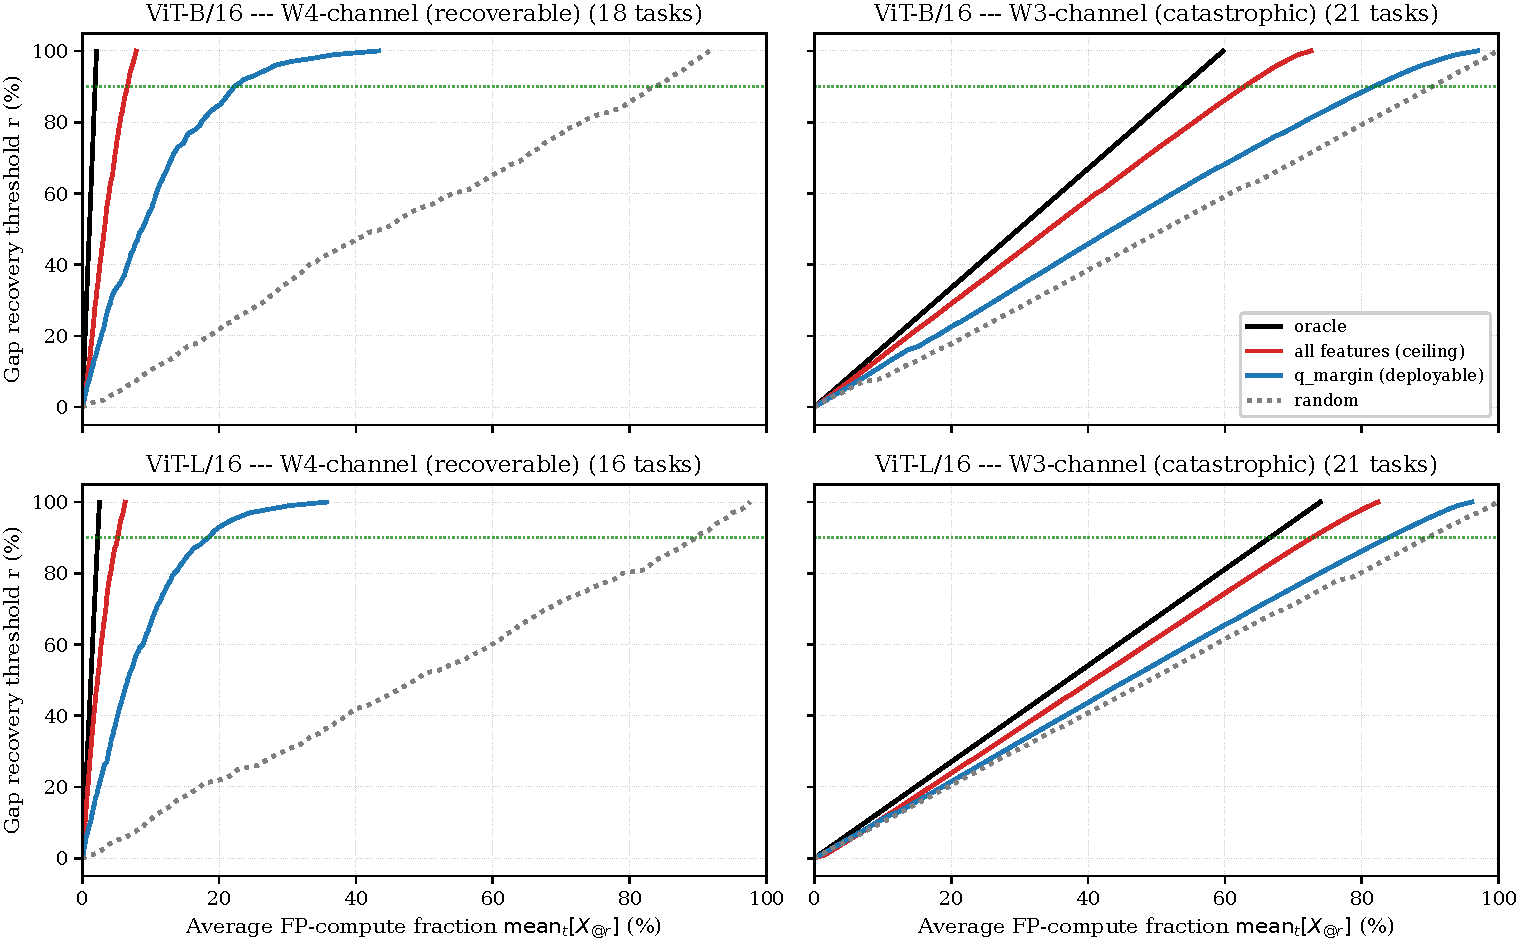
\includegraphics[width=\linewidth]{figs/fig_regime_comparison_dual_vit_base_patch16_224_orig_in21k_vs_vit_large_patch16_224_orig_in21k_W4vsW3_channel}
\caption{\textbf{Regime comparison: W4-channel (recoverable) vs.\ W3-channel (catastrophic) across backbone scales.} \textbf{Top row:} ViT-B/16. \textbf{Bottom row:} ViT-L/16. \textbf{Left:} W4-channel. \textbf{Right:} W3-channel. Same axes and aggregation as Figure~\ref{fig:headline}.}
\label{fig:regime}
\end{figure}

\paragraph{Implication for deployment shape.}
The \bad{}/\good{} ratio also flips at W3-channel: the \bad{} population grows from $\sim$5\% of test inputs at W4 to a strict majority at W3 ($\sim$62\% on ViT-B/16, $\sim$75\% on ViT-L/16; Table~\ref{tab:ablation_recipe}). Once \ptq{} is wrong on the majority of inputs, the deployment pattern this paper is about, cheap \ptq{} default with selective \fp{} fallback (\S\ref{sec:intro}), stops being the right shape, because the ``selective'' fallback would need to fire on most of the stream. This is a property of the regime itself, not the predictor: even perfect routing requires routing the majority of inputs to \fp{}. The deployable predictor's \xat{90} sitting near random on this regime is therefore signaling an inappropriate deployment use case, not a predictor failure of the method itself.

\paragraph{Recipe ablation: per-group scales relocate the recoverable boundary.}
The W3 catastrophe above is reported under per-channel RTN. A standard refinement is to assign one scale per contiguous block of 128 input features (six or eight scales per row instead of one), at no calibration or runtime cost: the same naive round-to-nearest applied to smaller chunks. We rerun the entire pipeline at $\mathrm{granularity}\!=\!\mathrm{group\_128}$ on all three backbones at both W4 and W3 (Table~\ref{tab:ablation_recipe}). Switching to per-group\_128 cuts the mean \fp$\to$\ptq{} gap at W3 by 54--78\% and the oracle's \xat{90} by 54--78\%; the offline X@90 of \texttt{q\_margin} becomes 43.8\% / 57.3\% / 46.0\% on ViT-B / ViT-L / Qwen3, meaningfully harder than W4 but no longer catastrophic (on ViT-B: 43.8\% routing / 90.2\% recovery, $\sigma\!=\!0.5$ pp across 20 tasks). The recoverable-regime boundary therefore sits at W3-group\_128 rather than at W4-channel: the W3 catastrophe is partly an artifact of naive per-channel RTN.

\begin{table}[t]
\centering
\caption{\textbf{Per-channel vs.\ per-group\_128 RTN at W4 and W3.} Mean over W4-eligible (top) and W3-eligible (bottom) tasks per backbone.}
\label{tab:ablation_recipe}
\small
\setlength{\tabcolsep}{4pt}
\begin{tabular}{lcccccc}
\toprule
& \multicolumn{2}{c}{ViT-B/16} & \multicolumn{2}{c}{ViT-L/16} & \multicolumn{2}{c}{Qwen3-Emb-0.6B} \\
\cmidrule(lr){2-3} \cmidrule(lr){4-5} \cmidrule(lr){6-7}
Metric & channel & group\_128 & channel & group\_128 & channel & group\_128 \\
\midrule
\multicolumn{7}{l}{\textit{W4 (recoverable regime)}} \\
n eligible tasks                & 18    & 17    & 16    & 13    & 9     & 9     \\
Mean \fp$\to$\ptq{} gap (pp)    & 2.1   & 1.3   & 2.3   & 0.7   & 2.0   & 0.8   \\
\texttt{q\_margin} \xat{90}     & 22.2\% & 17.5\% & 18.4\% & 9.4\%  & 20.2\% & 12.0\% \\
all\_features LOO \xat{90}      & 7.5\%  & 5.9\%  & 6.0\%  & 3.4\%  & 6.0\%  & 3.6\%  \\
oracle \xat{90}                 & 1.9\%  & 1.3\%  & 2.3\%  & 0.7\%  & 1.8\%  & 0.7\%  \\
\midrule
\multicolumn{7}{l}{\textit{W3 (was catastrophic under per-channel)}} \\
n eligible tasks                & 21    & 20    & 21    & 21    & 11    & 11    \\
Mean \fp$\to$\ptq{} gap (pp)    & 59.7  & 13.1  & 73.9  & 34.0  & 55.5  & 15.8  \\
\texttt{q\_margin} \xat{90}     & 81.7\%* & 43.8\% & 83.8\%* & 57.3\% & 83.4\%* & 46.0\% \\
all\_features LOO \xat{90}      & 65.7\%* & 20.1\% & 70.9\%* & 35.7\% & 57.3\%* & 20.2\% \\
oracle \xat{90}                 & 53.8\% & 11.8\% & 66.5\% & 30.6\% & 50.0\% & 14.2\% \\
\bottomrule
\end{tabular}
\flushleft\small\textit{*} Under per-channel W3 the deployable predictor sits within 2--7 pp of random's $\sim$90\% baseline; no recipe at the deployable end recovers compute.
\end{table}

\paragraph{Polarization with scale is recipe-invariant; the boundary location is not.}
At W4 on either recipe, ViT-L's eligible-task population shrinks relative to ViT-B (channel: 18~$\to$~16; group\_128: 17~$\to$~13). At W3 on either recipe, the oracle's \xat{90} climbs from ViT-B to ViT-L (channel: 53.8\%~$\to$~66.5\%; group\_128: 11.8\%~$\to$~30.6\%). Polarization survives the recipe change; the recoverable-boundary location does not. The deployable predictor adapts to either boundary with no protocol change. Per-group\_128 is a granularity refinement of naive RTN, not a different PTQ algorithm; state-of-the-art methods that additionally modify rounding (GPTQ, AWQ, SmoothQuant, QuaRot) would presumably extend the recoverable regime further but are beyond the scope of this work.

\end{document}